
\label{app}

\section{Image Difference and RGB Color}
To help explain the color difference plots later in the Appendix, it may be helpful to go into further depth on RGB (red, green,blue) based colors and how the individual values correspond to colors when mixed.

In the RGB color format, values for red, green, and blue can range from 0 to 255.  The higher the value for a color, the more of it is present in the resulting color.  If the values for red, green, and blue are the same, then the resulting color is a shade of grey.  If all values are set to their maximum, 255, then the result is pure white.  If all values are 0, then the result is pure black.  In general, colors with low RGB values are darker than  ones with greater RGB values.

To understand why the differences in the active core are in green (see Figure \ref{fig:120-180-diff} for an example), it is useful to revisit color theory and complementary colors.  The fission rate meshes are shown in a hot color map, which ranges in color from an almost-white shade of yellow, to very dark browns.  In between these maximum and minimum shades are varying shades of yellow, orange, and brown.  To create a shade of yellow in RGB format, one uses a large amount of red and green.  To create the sort of almost-white yellow, one simply takes the base yellow, with large amounts of red and green, and increases the blue value (which, as described before, will transition the color to a lighter shade as all three RGB values approach the maximum of 255).  To move from yellow to an orangey-brown, one shifts the green value down.  Lowering red and green while keeping blue at a low value produces the darkest shades of brown seen in the color map.

\begin{figure}[H]
\centering
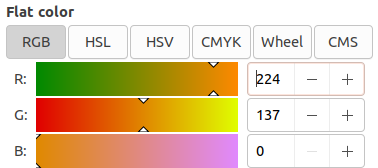
\includegraphics[width=0.6\linewidth]{figures/rgb-1}
\caption[An Example of RGB Color Values]{An example of RGB values.  If the value for red and blue are held constant, shifting the value for green up or down shifts the resulting color along the color gradient to the left of the green value, which ranges from red to yellow.  The arrows on the green gradient indicate what the current color is.  As one can see, moving the slider to the right - increasing the value of green - will make the color more yellow, while moving it to the left, or decreasing the green level, will shift it towards orange and red.}
\label{fig:rgb-1}
\end{figure}

Figure \ref{fig:rgb-1} gives an example of selecting a color using RGB values.  Image difference works by subtracting the RGB values from each other - for example, subtracting ( 200, 150, 50 ) from ( 100, 200, 75 ) results in ( 100, 50, 25 ).  Absolute values are used because negative values don't exist in RGB colors.  So, when  two colors which have contrasting values of green, and similar values of red and blue, the result is, of course, a shade of green.  The image difference results in the "banded" regions at the outermost edges of the active core shift to blue from green simply because in the original images this region is already in the yellow to white color range, and so the only RGB value that changes is blue.

One can image the two extremes that an image difference could give - pure black, or RGB (0, 0, 0) means the two images were identical at that particular pixel.  Meanwhile, pure white --- (255, 255, 255) --- is the greatest possible difference that could exist.  Therefore, when interpreting the image difference results in Appendix A and Appendix B, it is important to keep in mind that the specific \emph{color} the differences are shown in --- usually green, but also blue or, rarely, red --- are far less important than how bright, or intense, these colors are.

\section{Appendix A: Symmetry Test}
\label{app-sym}

Appendix A contains the geometry cross sections, fission rate/thermal flux meshes, and image difference results from the other symmetry tests, corresponding to Run 2 through Run 5 in Figure \ref{fig:slicetest}.  These symmetry test use an otherwise identical core model and set of run parameters (see \autoref{sec-run-params}) for the Sangamon20 core model.  Image difference for each run compares to the Sangamon20 control model results.


\begin{figure}[h!]
\centering

\begin{subfigure}{0.45\textwidth}
  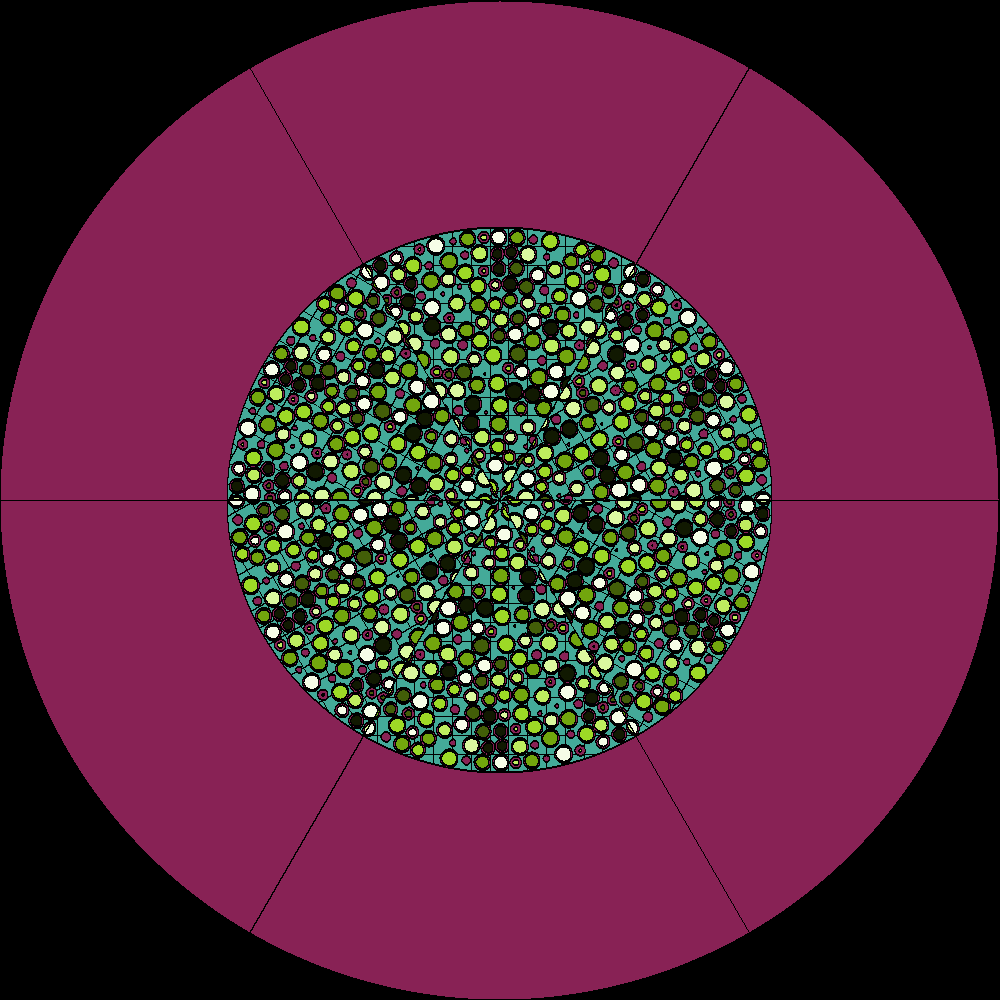
\includegraphics[width=0.95\linewidth]{figures/60-120/60-120-r}
  \caption{Radial Cross Section at y=0}
  \label{fig:bstep0}
\end{subfigure}%
%
\begin{subfigure}{0.45\textwidth}
  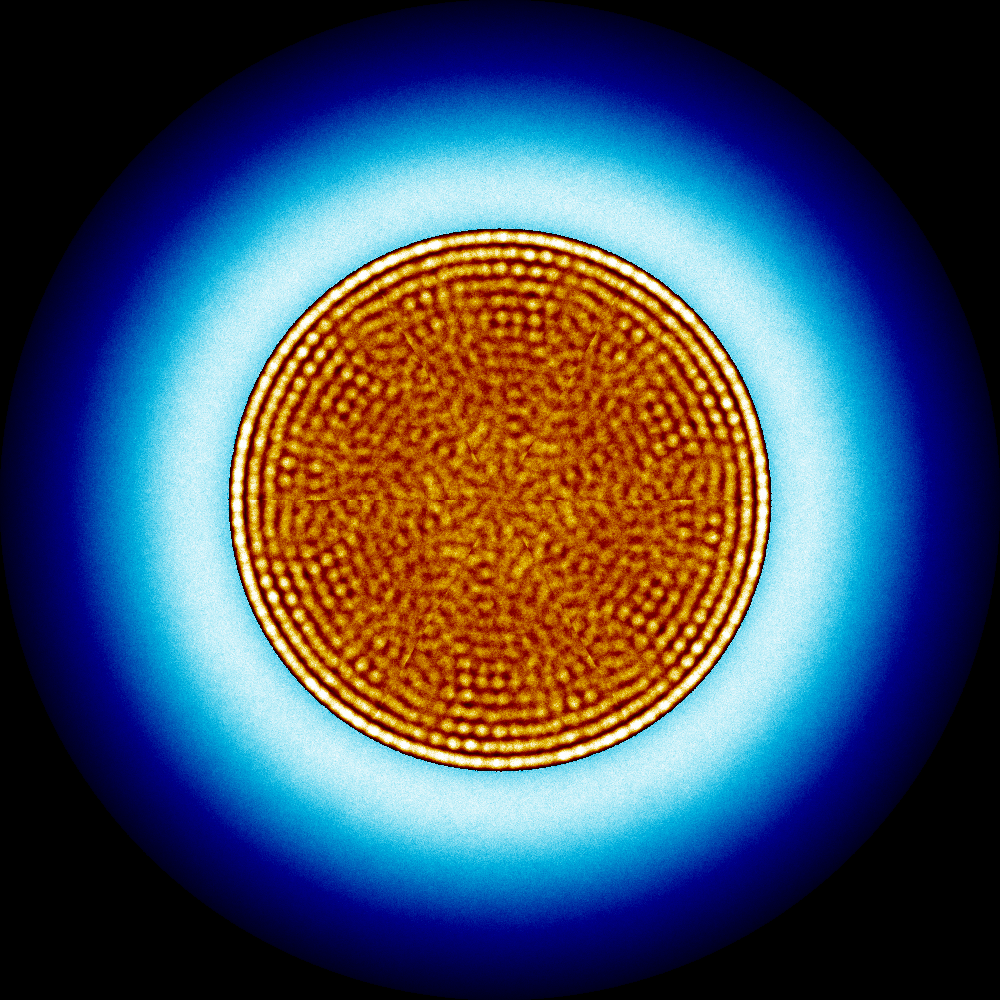
\includegraphics[width=0.95\linewidth]{figures/60-120/60-120-rm}
  \caption{Radial Mesh}
  \label{fig:bstep1}
\end{subfigure}

\begin{subfigure}{0.45\textwidth}
  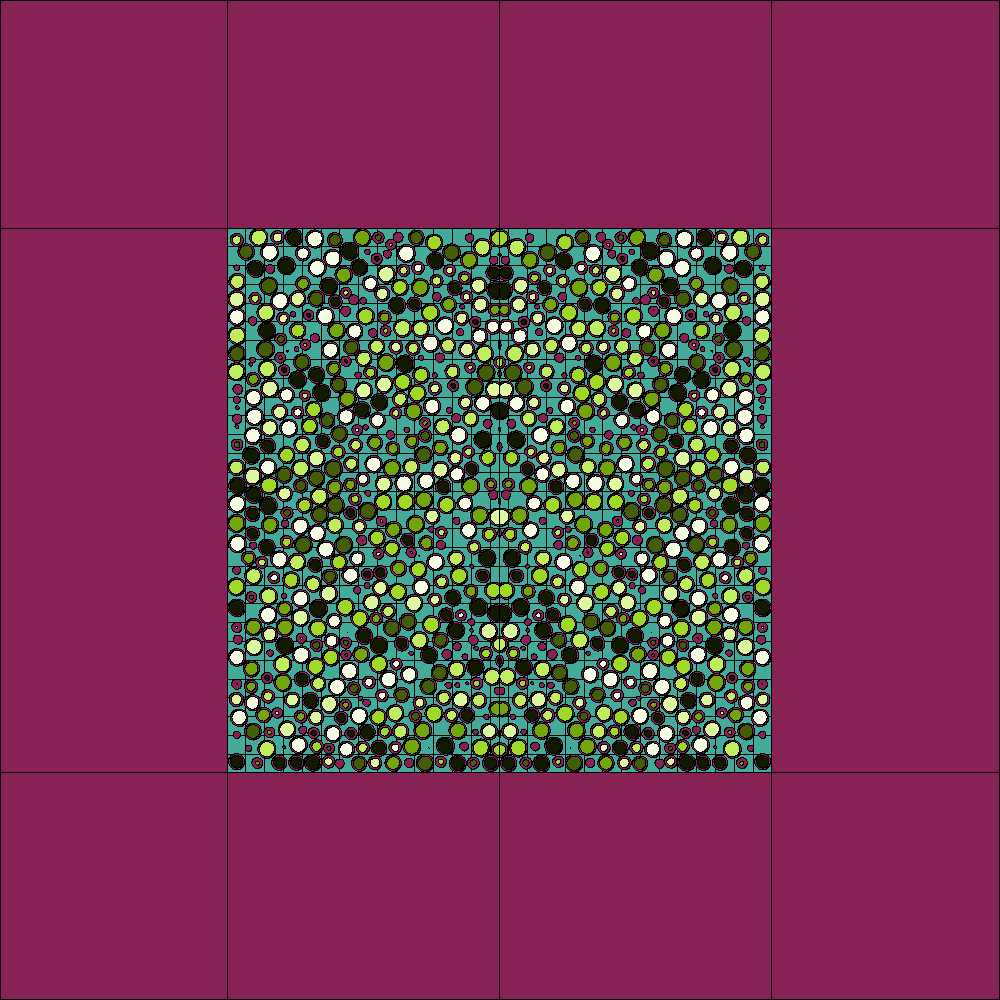
\includegraphics[width=0.95\linewidth]{figures/60-120/60-120-v}
  \caption{Axial Cross Section at z=0 }
  \label{fig:bstep1}
\end{subfigure}
%
\begin{subfigure}{0.45\textwidth}
  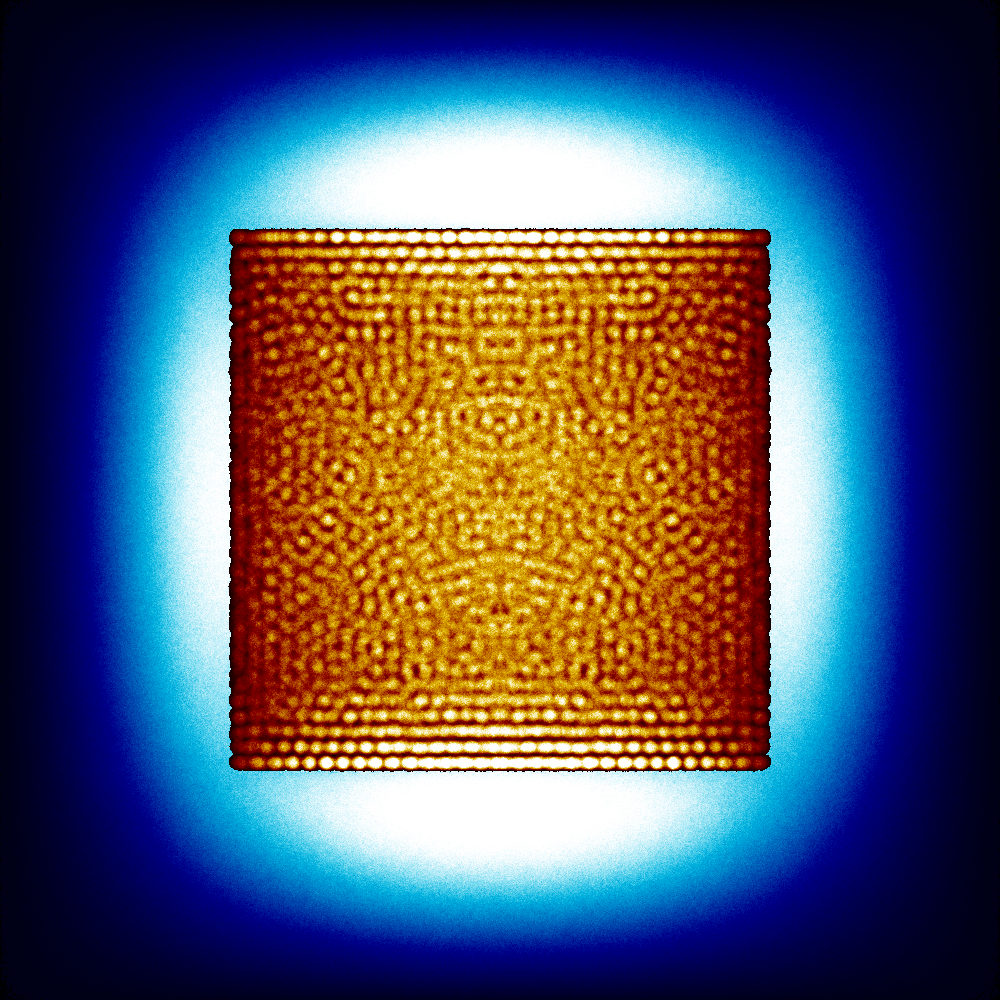
\includegraphics[width=0.95\linewidth]{figures/60-120/60-120-vm}
  \caption{Axial Mesh}
  \label{fig:bstep1}
\end{subfigure}
%
\caption{Sensitivity Analysis: $60^{\circ}$ - $120^{\circ}$}
\label{fig:60-120}
\end{figure}
\begin{figure}[H]
\centering
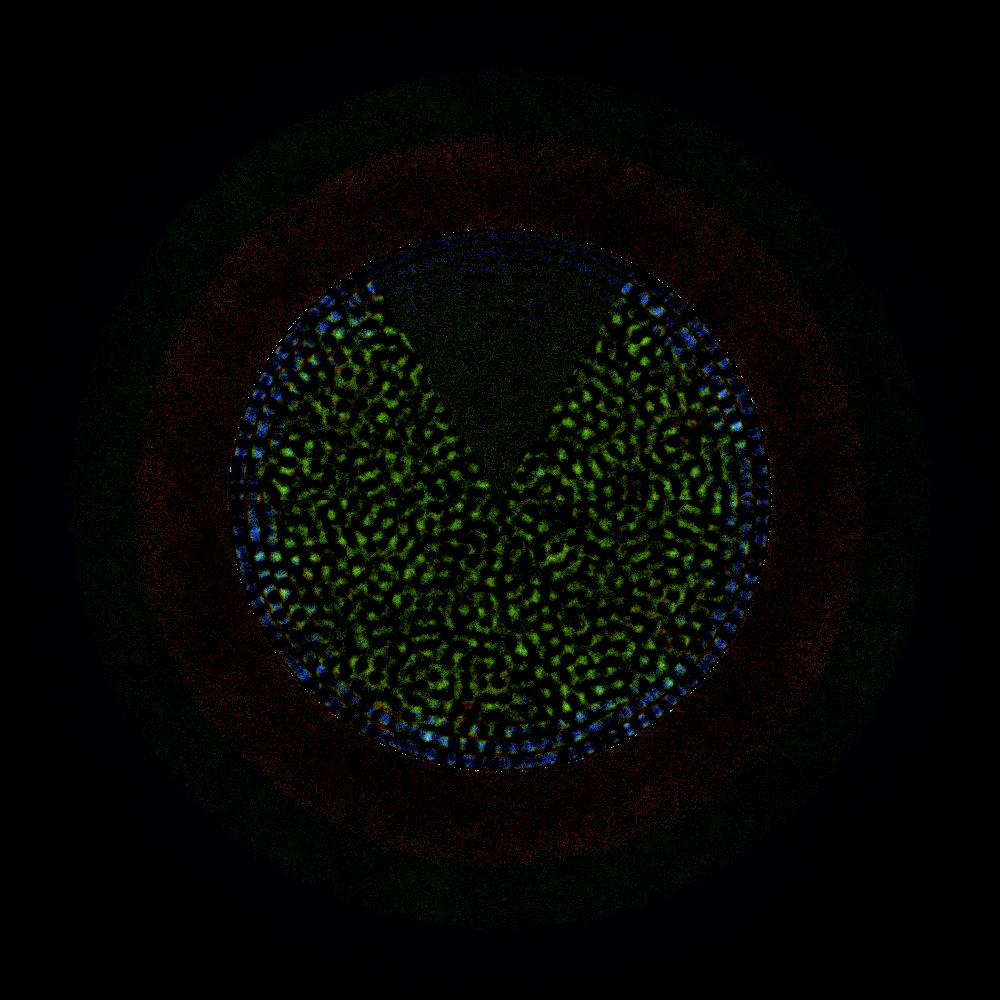
\includegraphics[width=0.6\linewidth]{figures/60-120/diff-60-120}
\caption{An Image Generated by Subtracting Figure \ref{fig:60-120-rm} from Figure \ref{fig:controlb}.}
\label{fig:60-120-diff}
\end{figure}

Figure \ref{fig:60-120} provides fission rate and thermal flux visualization meshes for the symmetry test using the 60 - 120 degree slice.  Figure \ref{fig:60-120-diff} is the result of using image-difference between the control's full-core radial mesh and the symmetry test's mesh.

\begin{figure}[H]
\centering

\begin{subfigure}{0.45\textwidth}
  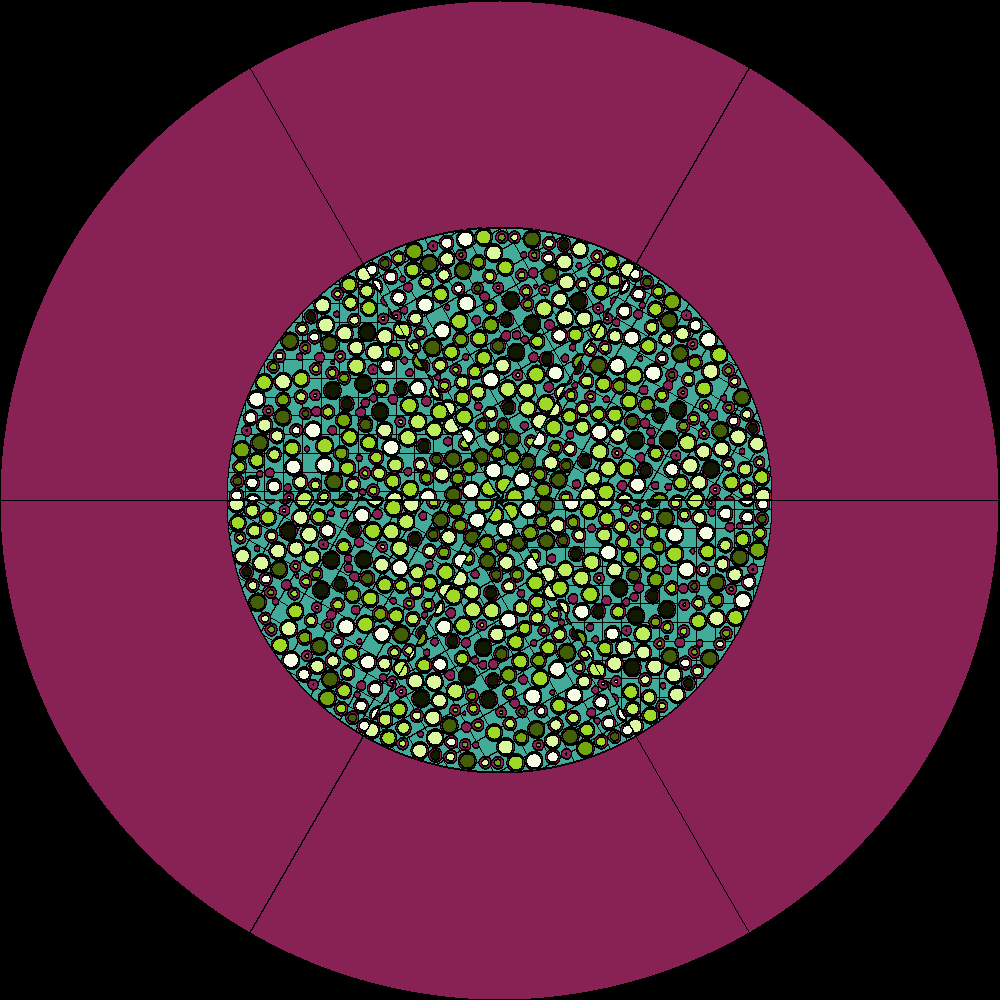
\includegraphics[width=0.95\linewidth]{figures/120-180/120-180-r}
  \caption{Radial Cross Section at y=0}
  \label{fig:120-180-r}
\end{subfigure}%
%
\begin{subfigure}{0.45\textwidth}
  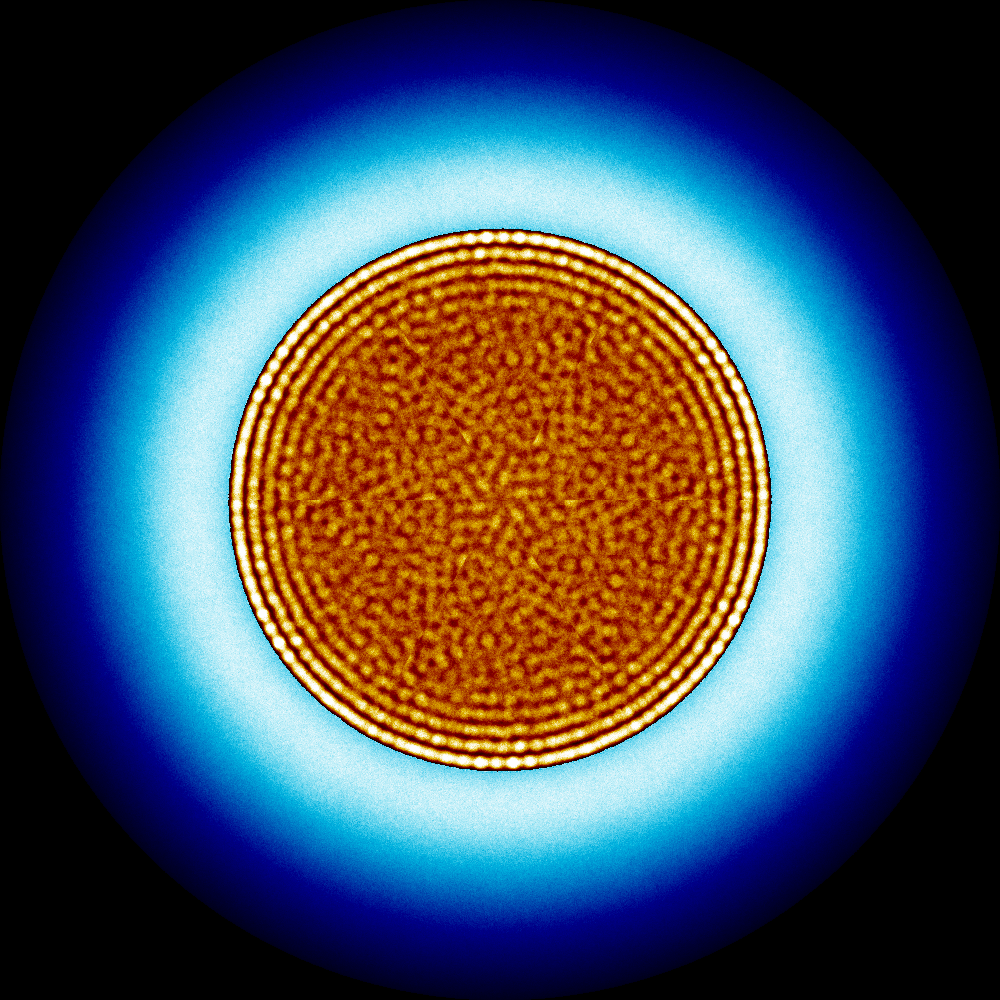
\includegraphics[width=0.95\linewidth]{figures/120-180/120-180-rm}
  \caption{Radial Mesh}
  \label{fig:120-180-rm}
\end{subfigure}

\begin{subfigure}{0.45\textwidth}
  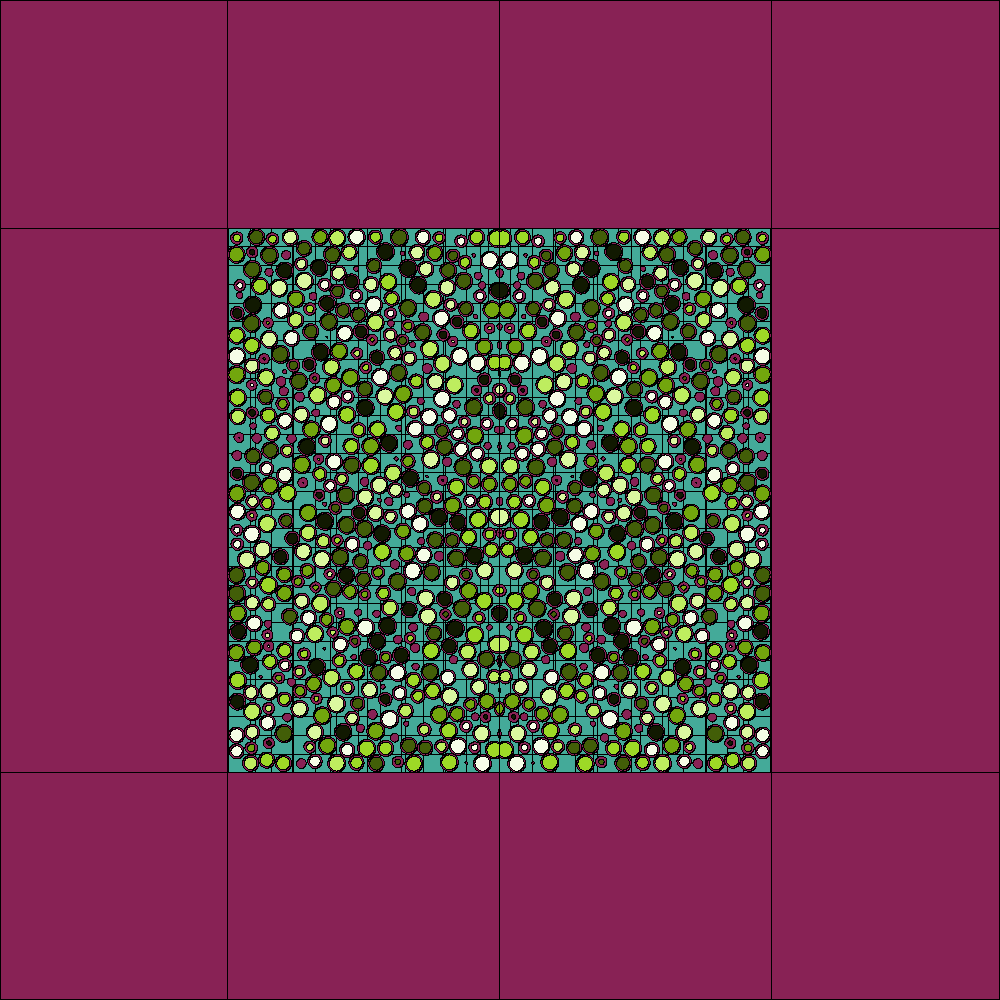
\includegraphics[width=0.95\linewidth]{figures/120-180/120-180-v}
  \caption{Axial Cross Section at z=0 }
  \label{fig:120-180-v}
\end{subfigure}
%
\begin{subfigure}{0.45\textwidth}
  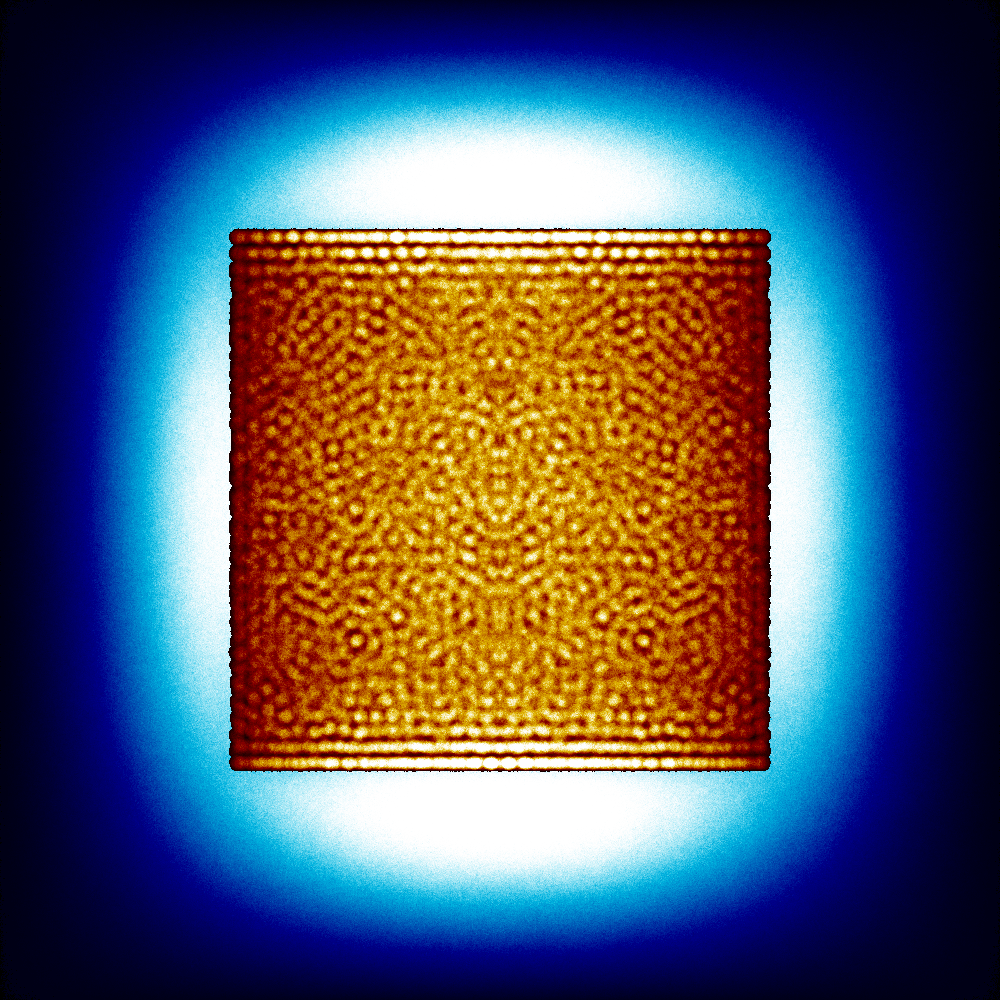
\includegraphics[width=0.95\linewidth]{figures/120-180/120-180-vm}
  \caption{Axial Mesh}
  \label{fig:120-180-vm}
\end{subfigure}
%
\caption{Sensitivity Analysis: $120^{\circ}$ - $180^{\circ}$}
\label{fig:120-180}
\end{figure}
\begin{figure}[H]
\centering
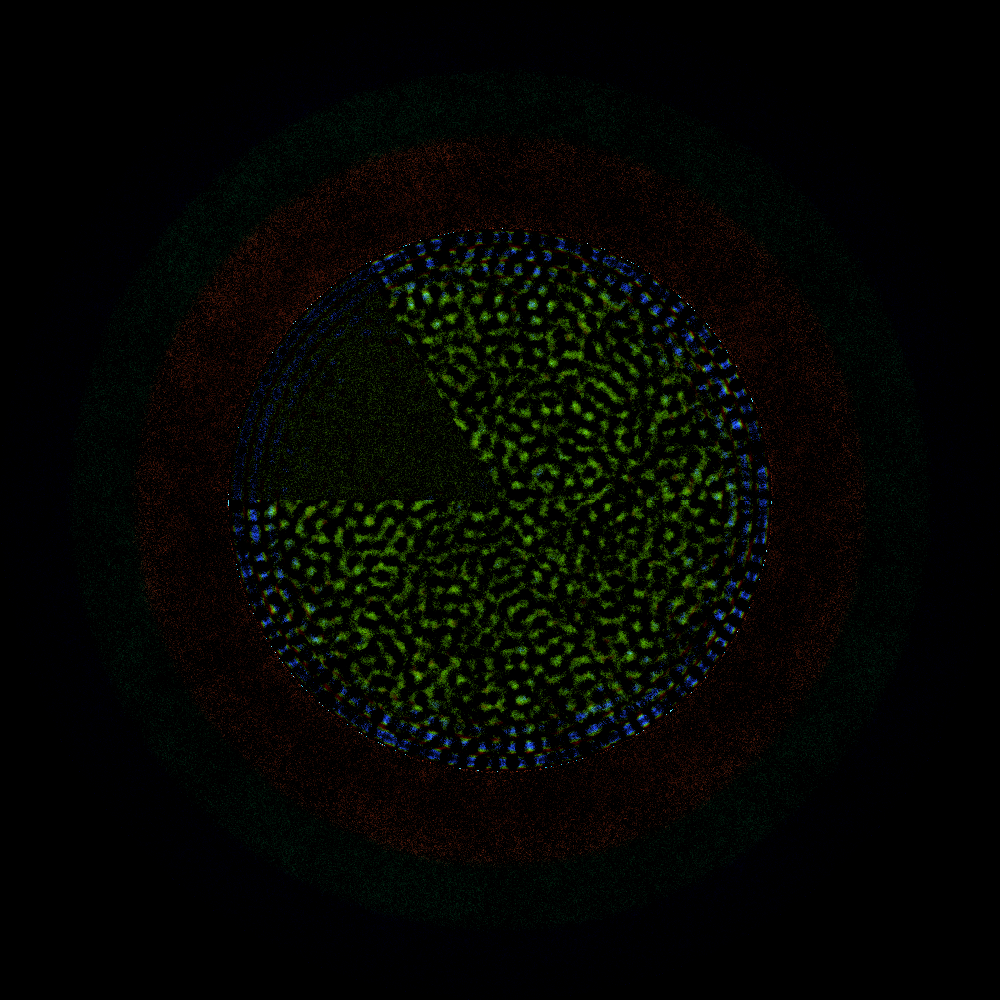
\includegraphics[width=0.6\linewidth]{figures/120-180/diff-120-180}
\caption{An Image Generated by Subtracting \ref{fig:120-180-rm} from \ref{fig:controlb}.}
\label{fig:120-180-diff}
\end{figure}

Figure \ref{fig:120-180} provides fission rate and thermal flux visualization meshes for the symmetry test using the 120 - 180 degree slice.  Figure \ref{fig:120-180-diff} is the result of using image-difference between the control's full-core radial mesh and the symmetry test's mesh.

\begin{figure}
\centering

\begin{subfigure}{0.45\textwidth}
  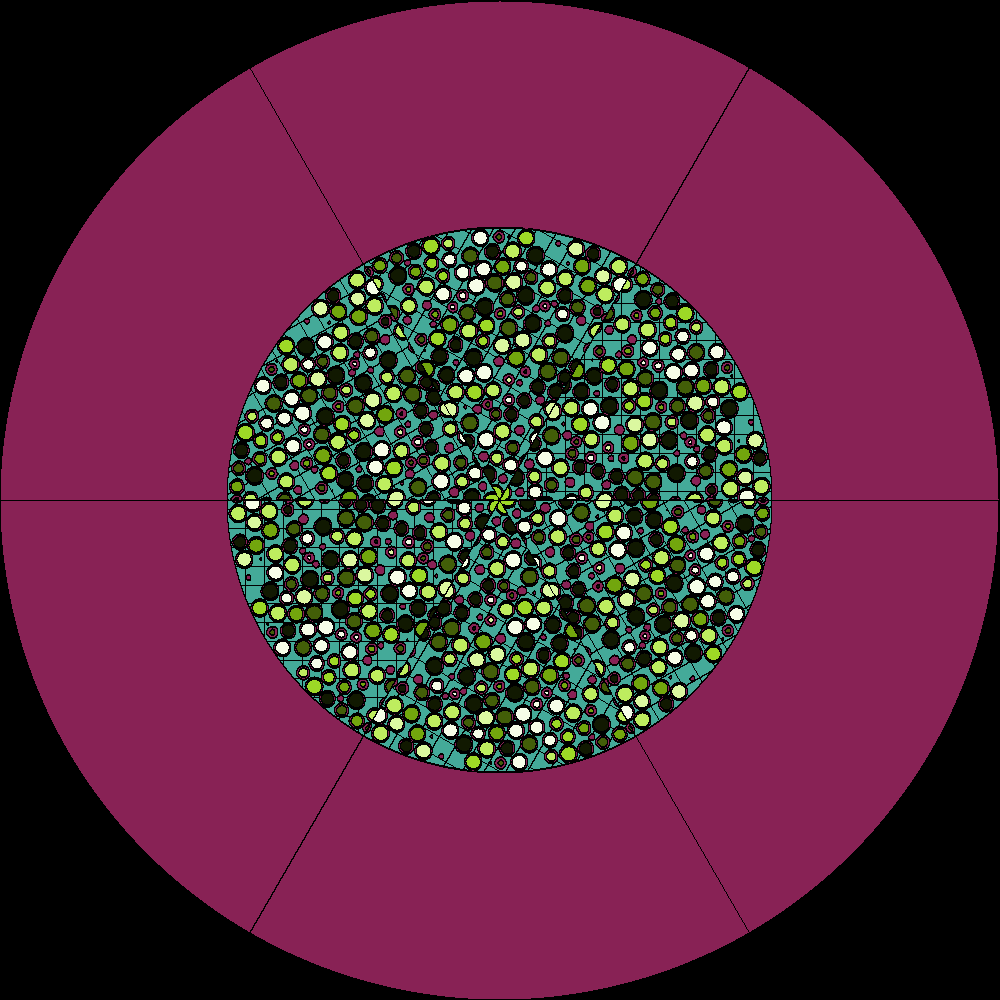
\includegraphics[width=0.95\linewidth]{figures/180-240/180-240-r}
  \caption{Radial Cross Section at y=0}
  \label{fig:bstep0}
\end{subfigure}%
%
\begin{subfigure}{0.45\textwidth}
  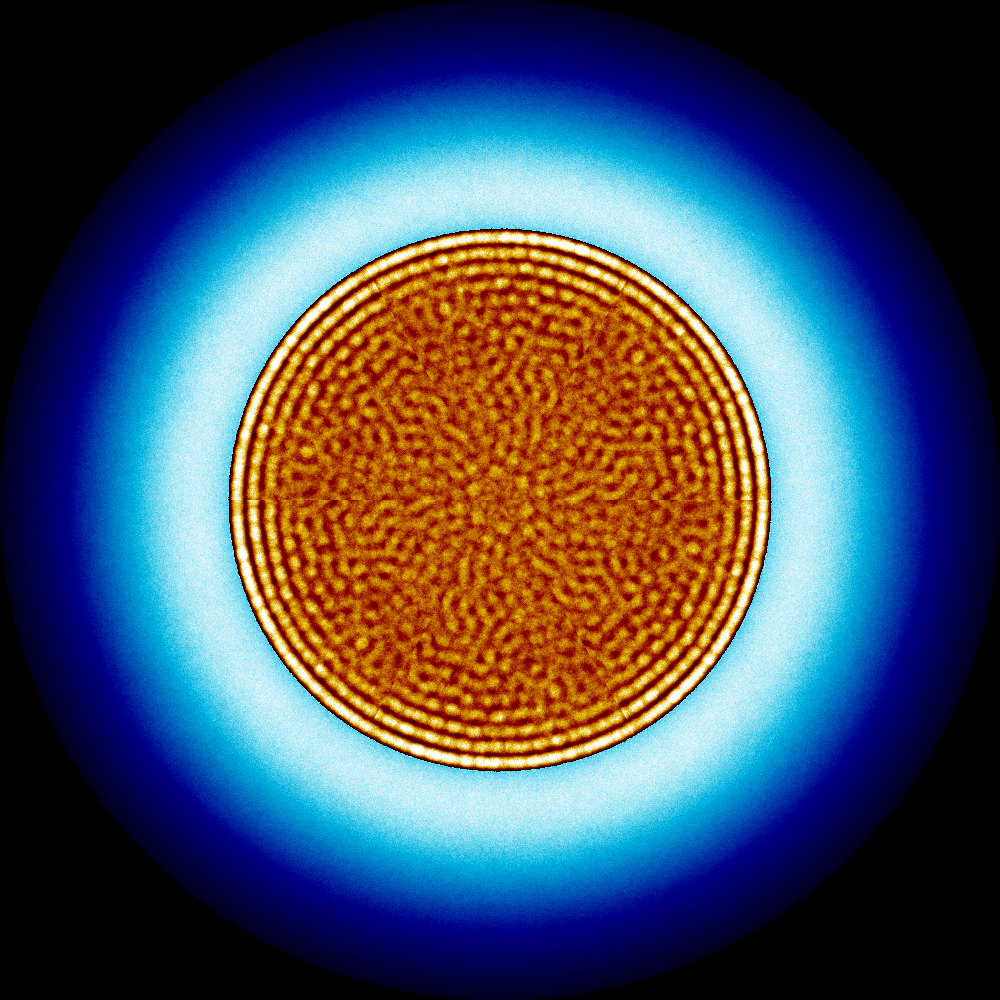
\includegraphics[width=0.95\linewidth]{figures/180-240/180-240-rm}
  \caption{Radial Mesh}
  \label{fig:bstep1}
\end{subfigure}

\begin{subfigure}{0.45\textwidth}
  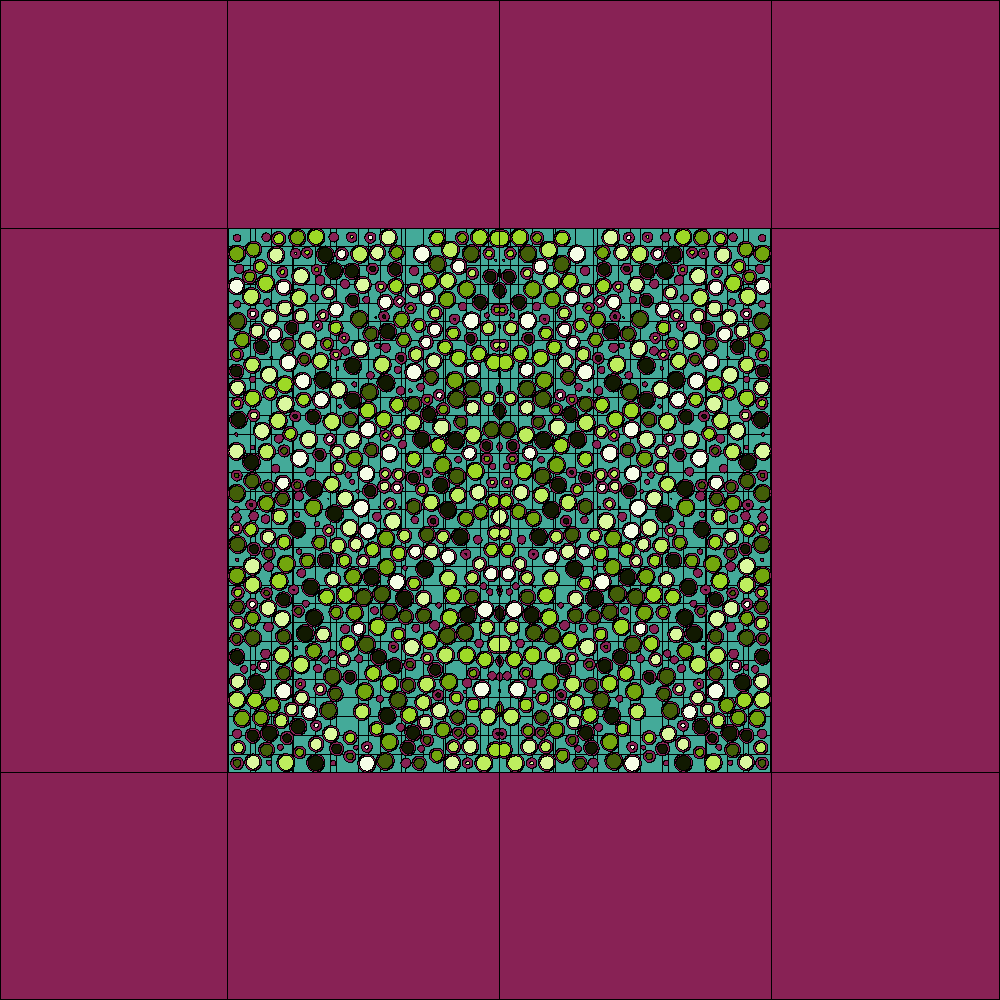
\includegraphics[width=0.95\linewidth]{figures/180-240/180-240-v}
  \caption{Axial Cross Section at z=0 }
  \label{fig:bstep1}
\end{subfigure}
%
\begin{subfigure}{0.45\textwidth}
  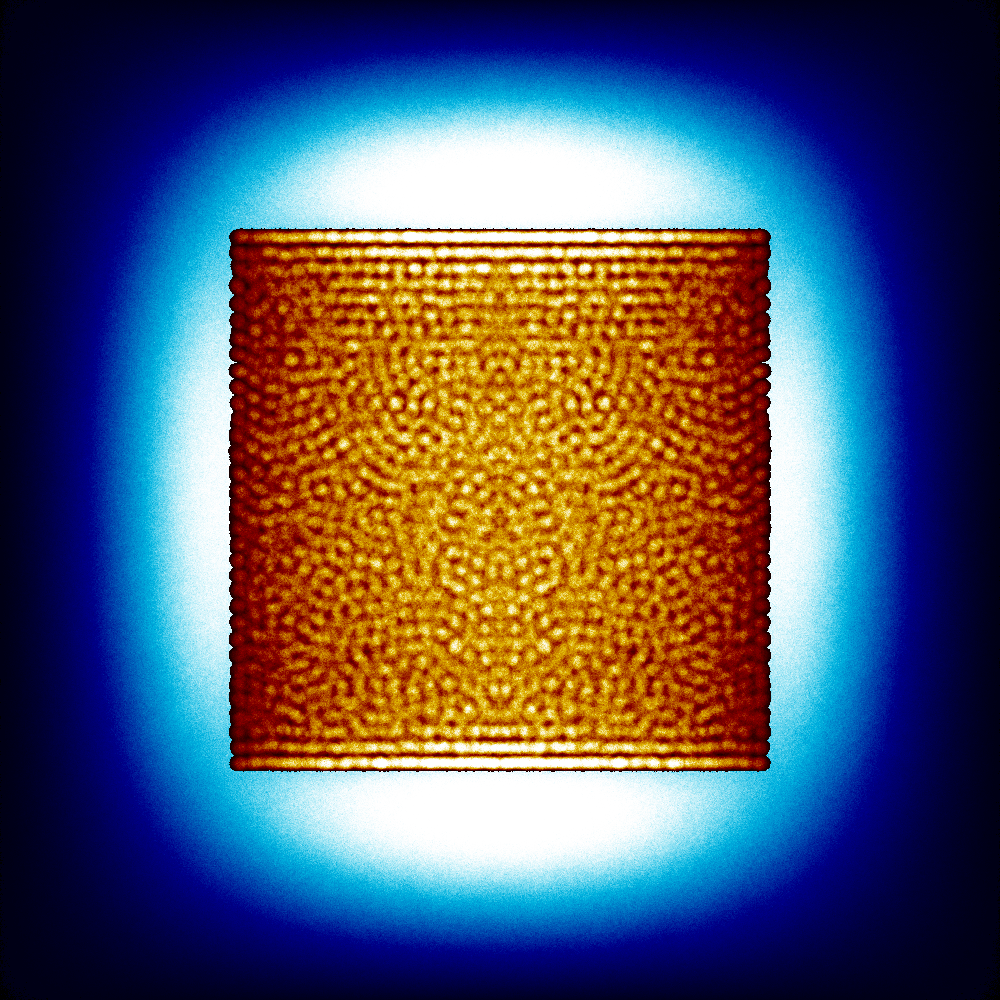
\includegraphics[width=0.95\linewidth]{figures/180-240/180-240-vm}
  \caption{Axial Mesh}
  \label{fig:bstep1}
\end{subfigure}
%
\caption{Sensitivity Analysis: $180^{\circ}$ - $240^{\circ}$}
\label{fig:180-240}
\end{figure}
\begin{figure}[H]
\centering
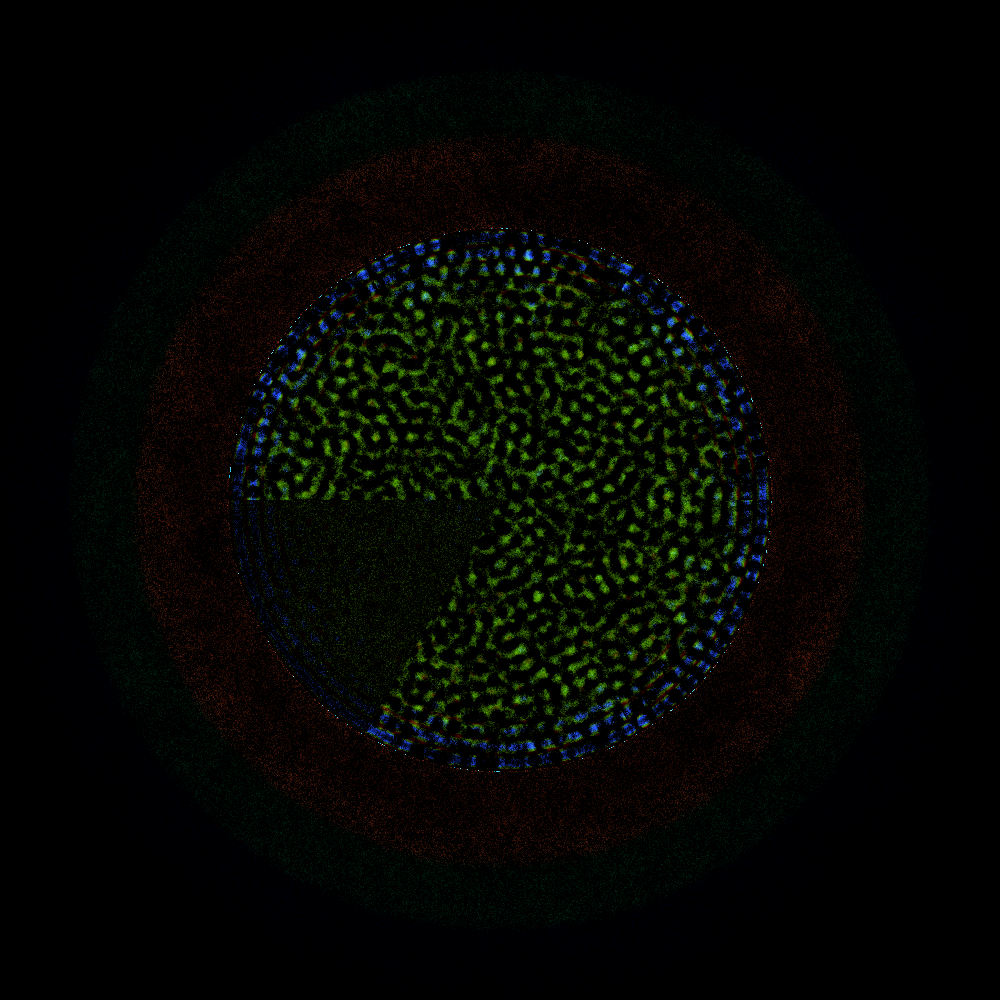
\includegraphics[width=0.6\linewidth]{figures/180-240/diff-180-240}
\caption{An Image Generated by Subtracting Figure \ref{fig:180-240-rm} from Figure \ref{fig:controlb}.}
\label{fig:180-240-diff}
\end{figure}

Figure \ref{fig:180-240} provides fission rate and thermal flux visualization meshes for the symmetry test using the 180 - 240 degree slice.  Figure \ref{fig:180-240-diff} is the result of using image-difference between the control's full-core radial mesh and the symmetry test's mesh.

\begin{figure}
\centering

\begin{subfigure}{0.45\textwidth}
  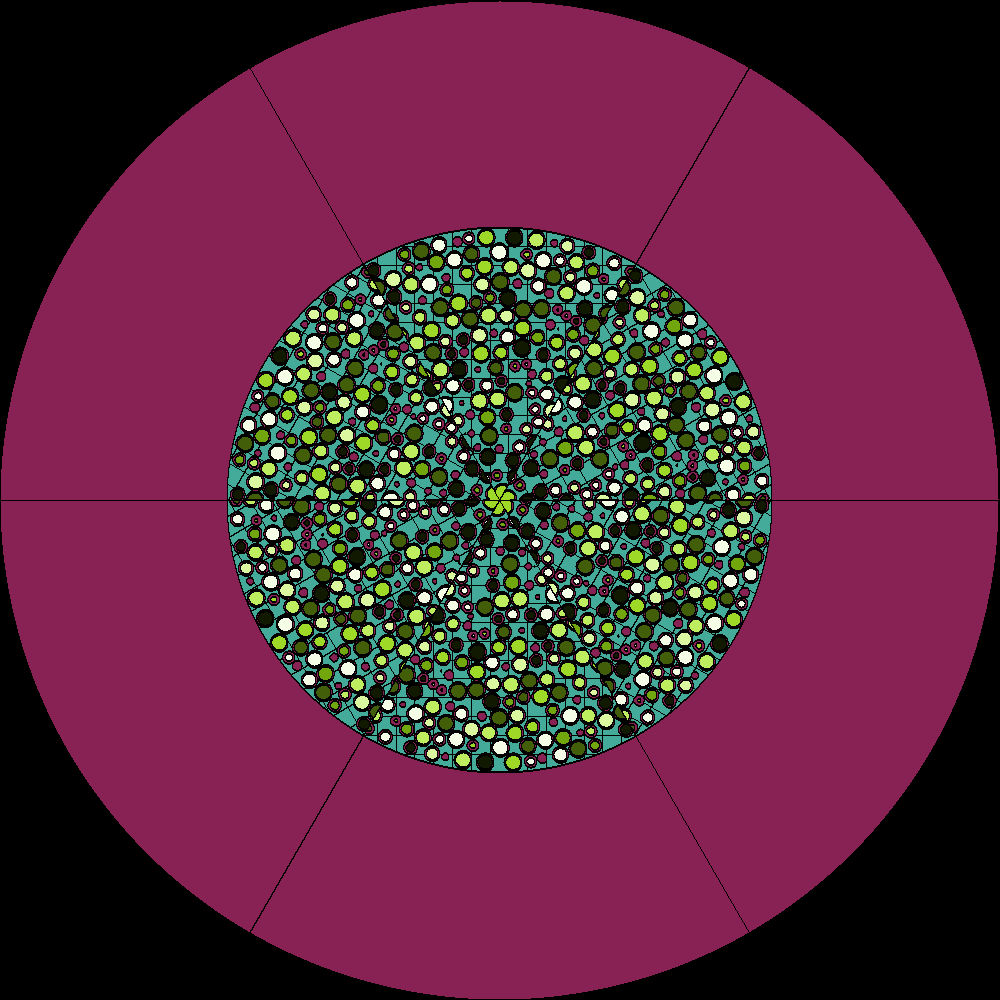
\includegraphics[width=0.95\linewidth]{figures/240-300/240-300-r}
  \caption{Radial Cross Section at y=0}
  \label{fig:bstep0}
\end{subfigure}%
%
\begin{subfigure}{0.45\textwidth}
  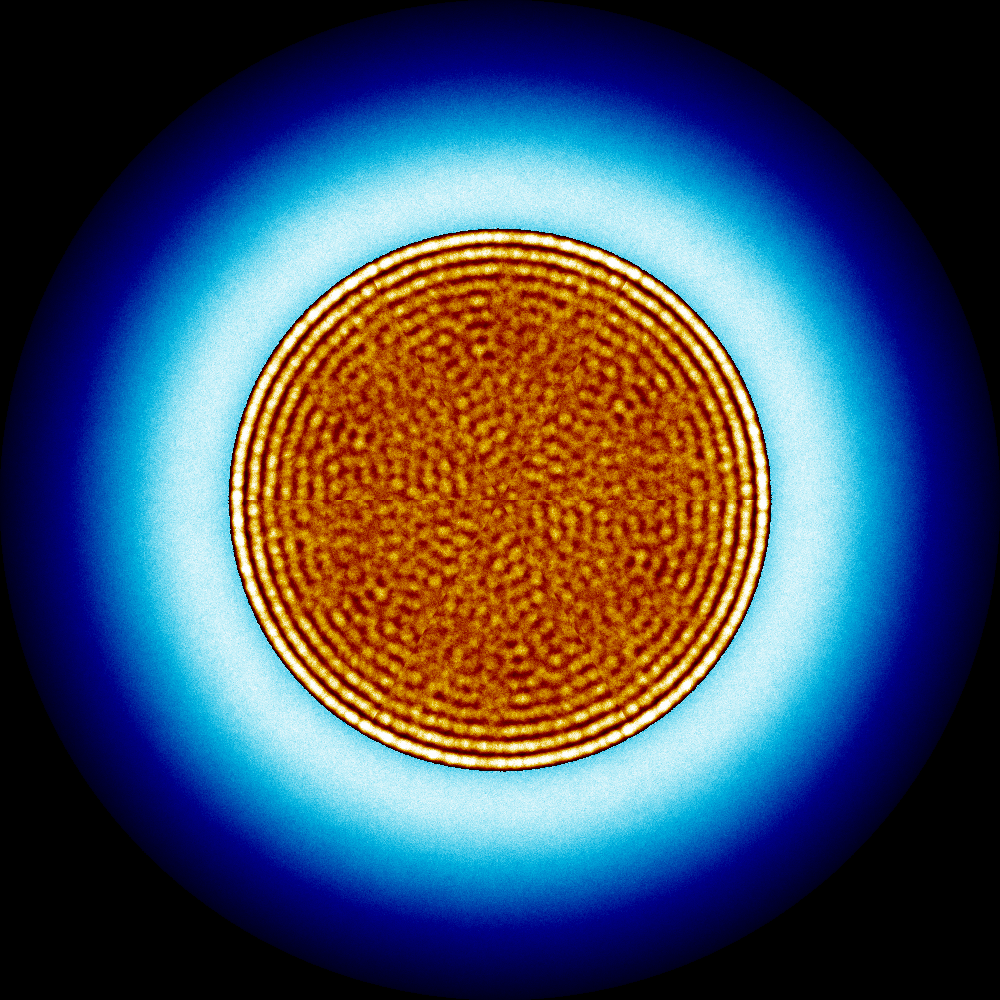
\includegraphics[width=0.95\linewidth]{figures/240-300/240-300-rm}
  \caption{Radial Mesh}
  \label{fig:bstep1}
\end{subfigure}

\begin{subfigure}{0.45\textwidth}
  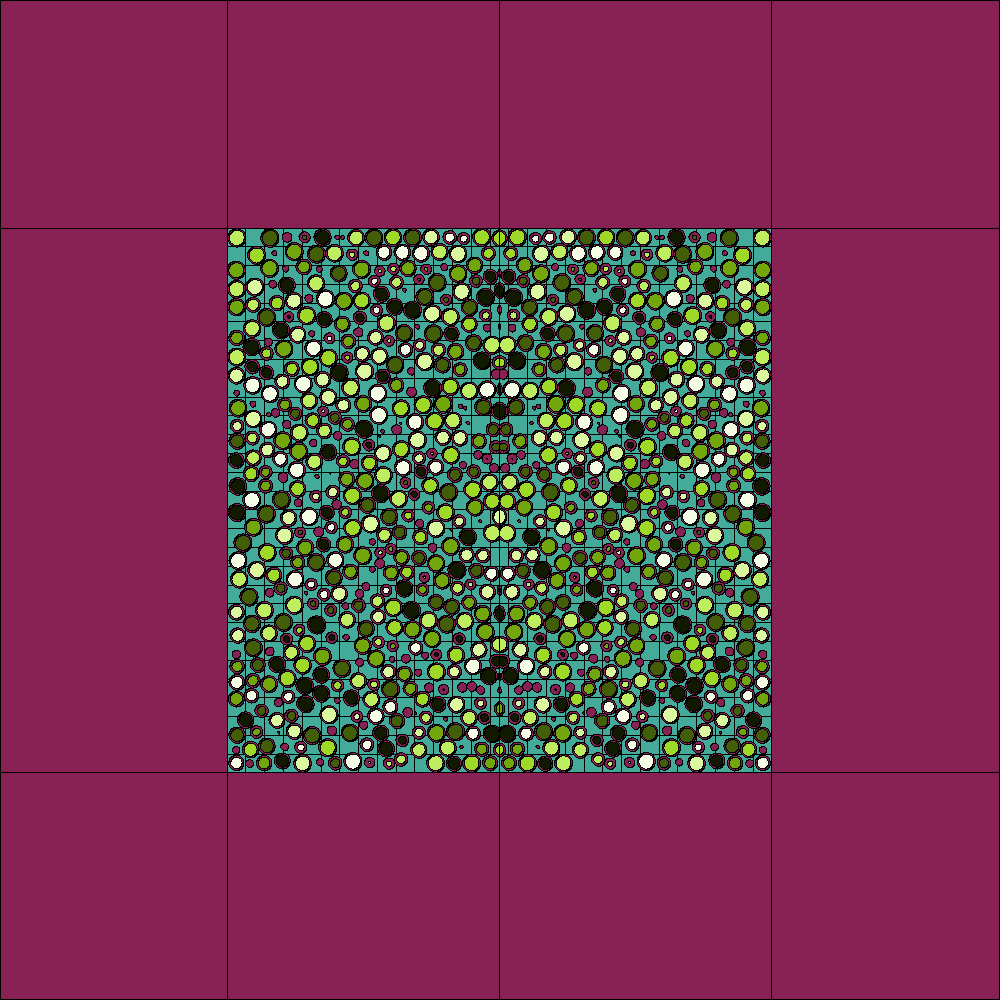
\includegraphics[width=0.95\linewidth]{figures/240-300/240-300-v}
  \caption{Axial Cross Section at z=0 }
  \label{fig:bstep1}
\end{subfigure}
%
\begin{subfigure}{0.45\textwidth}
  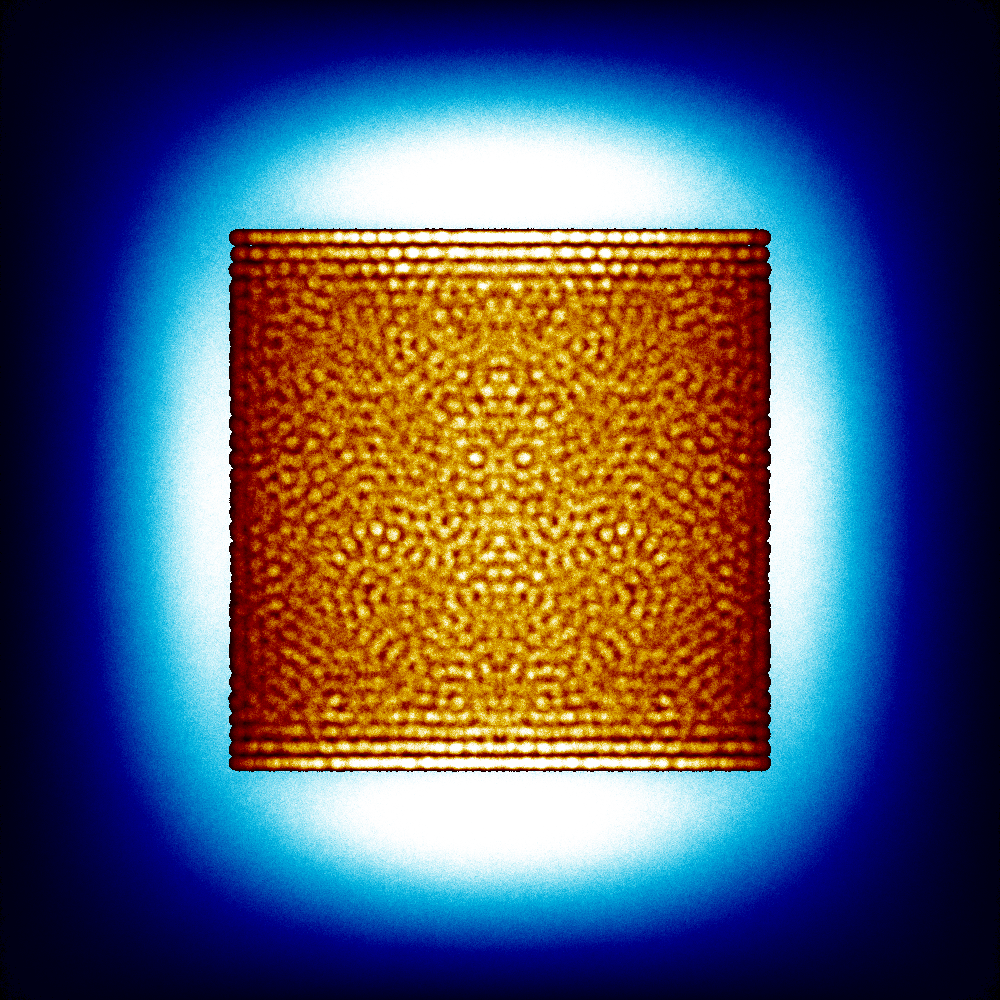
\includegraphics[width=0.95\linewidth]{figures/240-300/240-300-vm}
  \caption{Axial Mesh}
  \label{fig:bstep1}
\end{subfigure}
%
\caption{Sensitivity Analysis: $240^{\circ}$ - $300^{\circ}$}
\label{fig:240-300}
\end{figure}
\begin{figure}[H]
\centering
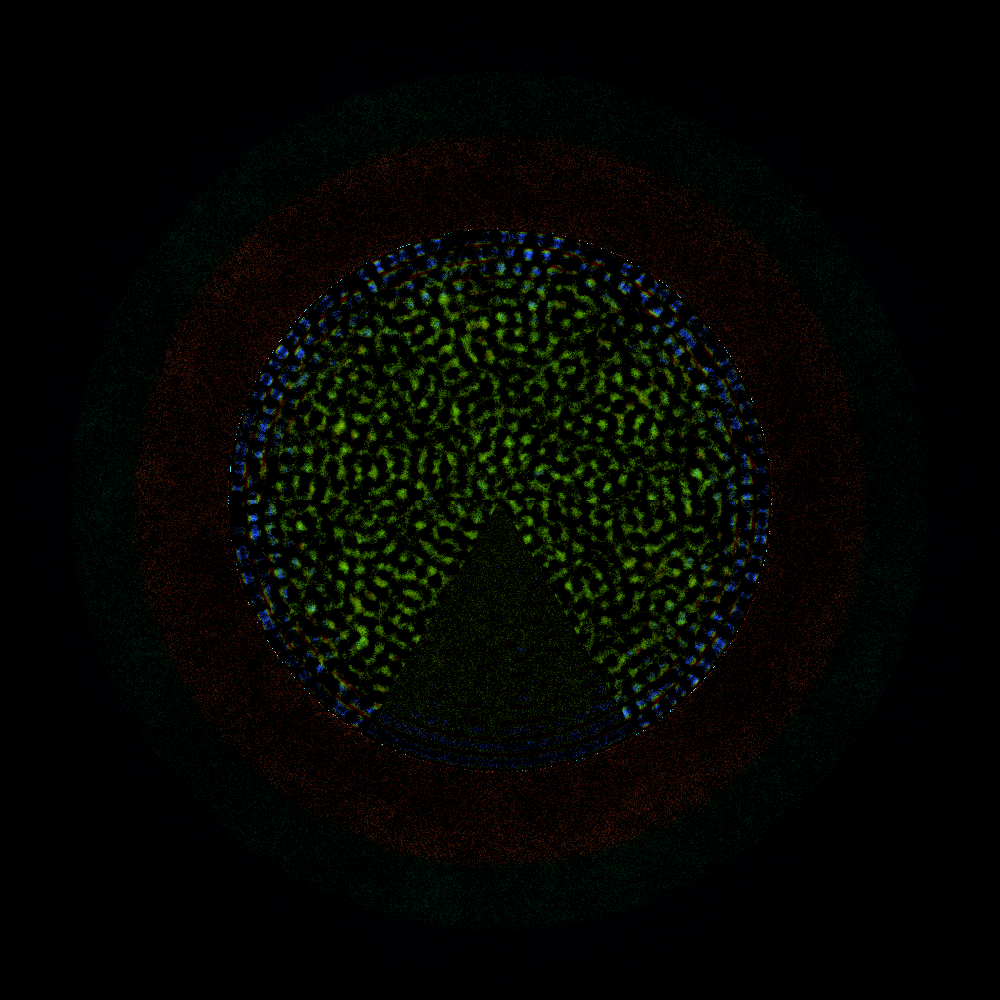
\includegraphics[width=0.6\linewidth]{figures/240-300/diff-240-300}
\caption{An Image Generated by Subtracting Figure \ref{fig:240-300-rm} from Figure \ref{fig:controlb}.}
\label{fig:240-300-diff}
\end{figure}

Figure \ref{fig:240-300} provides fission rate and thermal flux visualization meshes for the symmetry test using the 240 - 300 degree slice.  Figure \ref{fig:240-300-diff} is the result of using image-difference between the control's full-core radial mesh and the symmetry test's mesh.

\begin{figure}[H]
\centering

\begin{subfigure}{0.45\textwidth}
  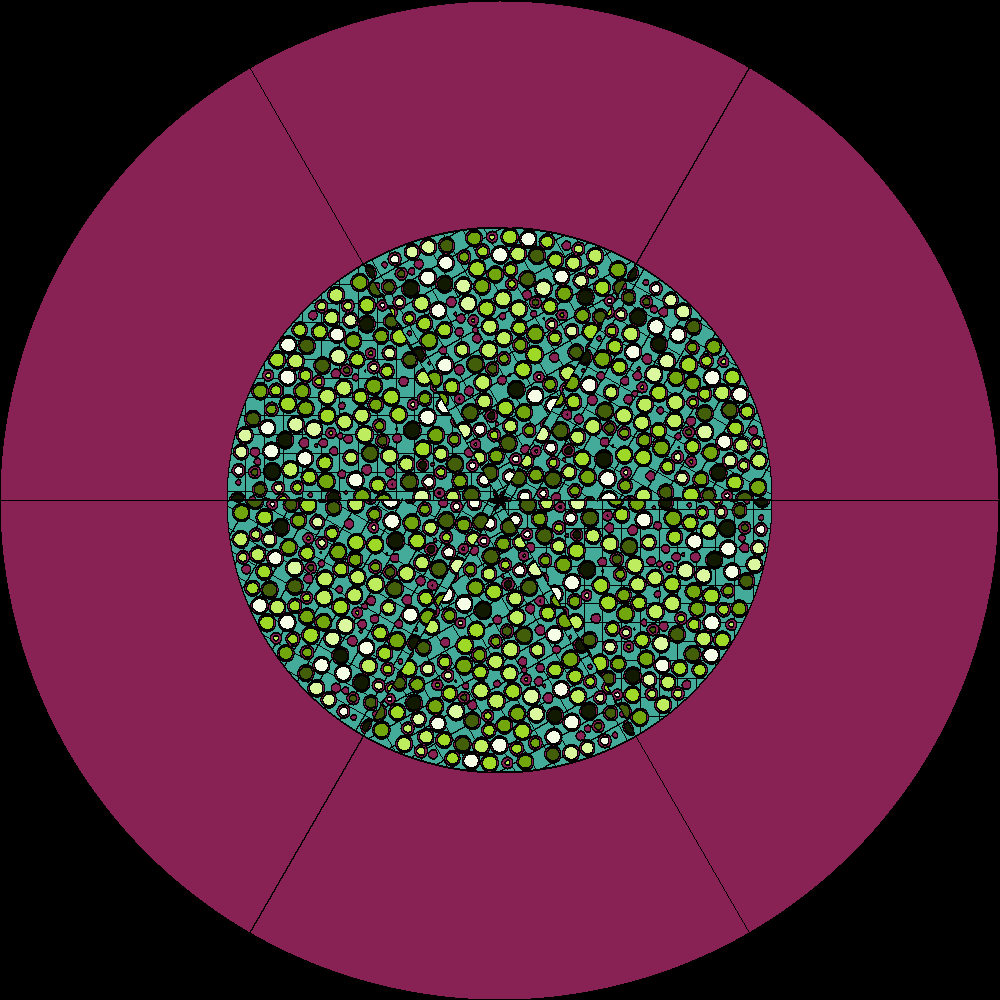
\includegraphics[width=0.95\linewidth]{figures/300-360/300-360-r}
  \caption{Radial Cross Section at y=0}
  \label{fig:bstep0}
\end{subfigure}%
%
\begin{subfigure}{0.45\textwidth}
  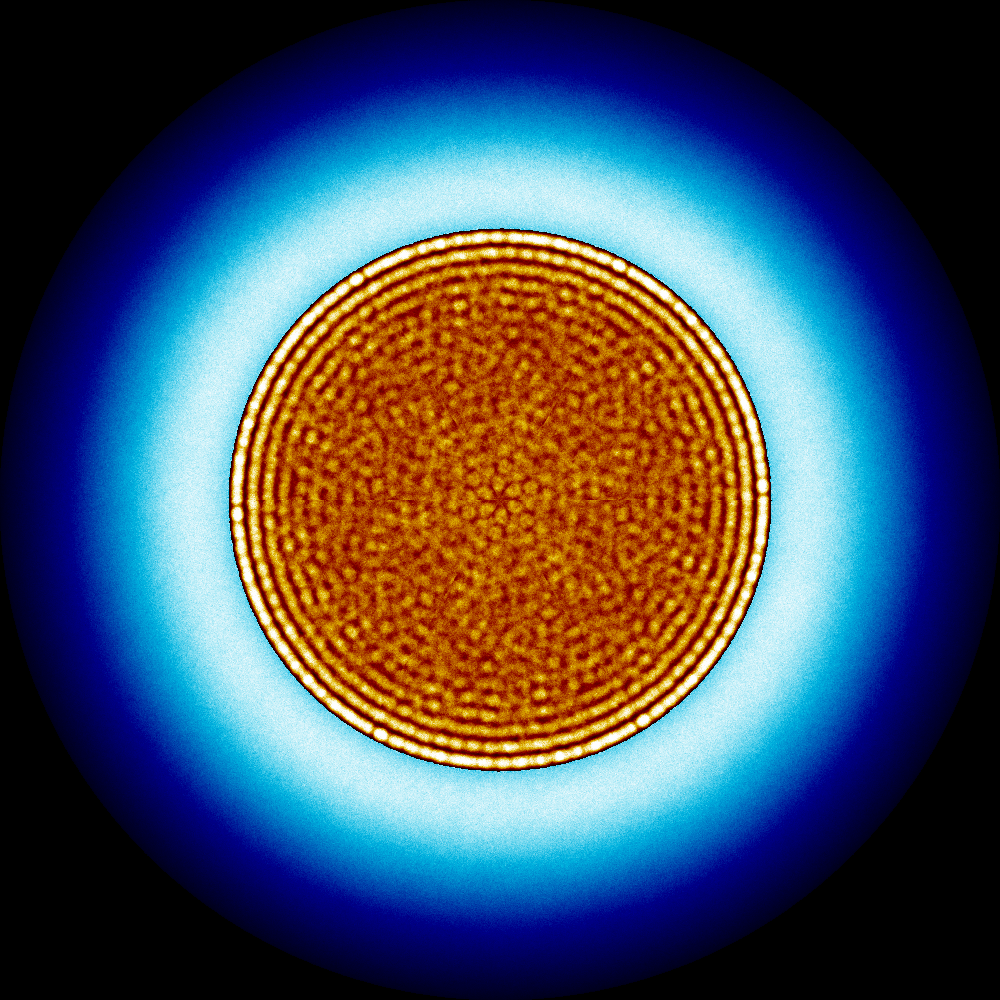
\includegraphics[width=0.95\linewidth]{figures/300-360/300-360-rm}
  \caption{Radial Mesh}
  \label{fig:bstep1}
\end{subfigure}

\begin{subfigure}{0.45\textwidth}
  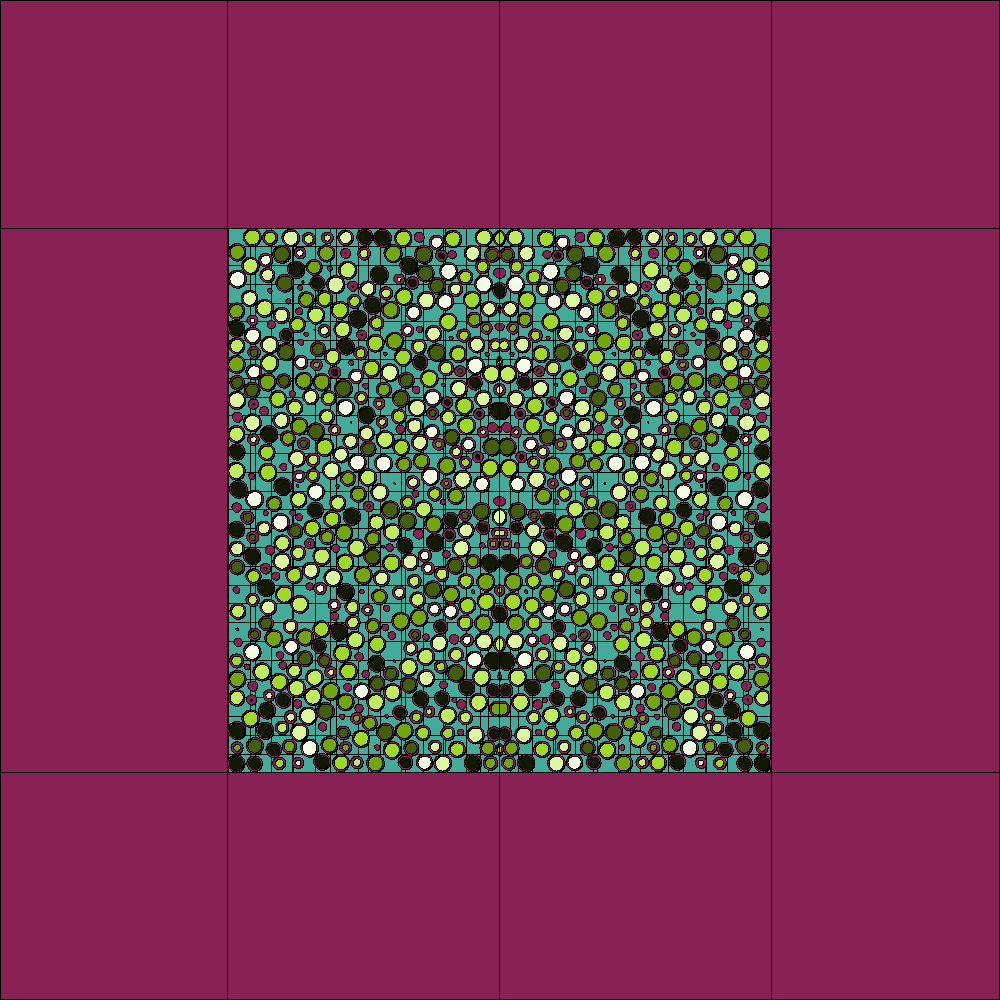
\includegraphics[width=0.95\linewidth]{figures/300-360/300-360-v}
  \caption{Axial Cross Section at z=0 }
  \label{fig:bstep1}
\end{subfigure}
%
\begin{subfigure}{0.45\textwidth}
  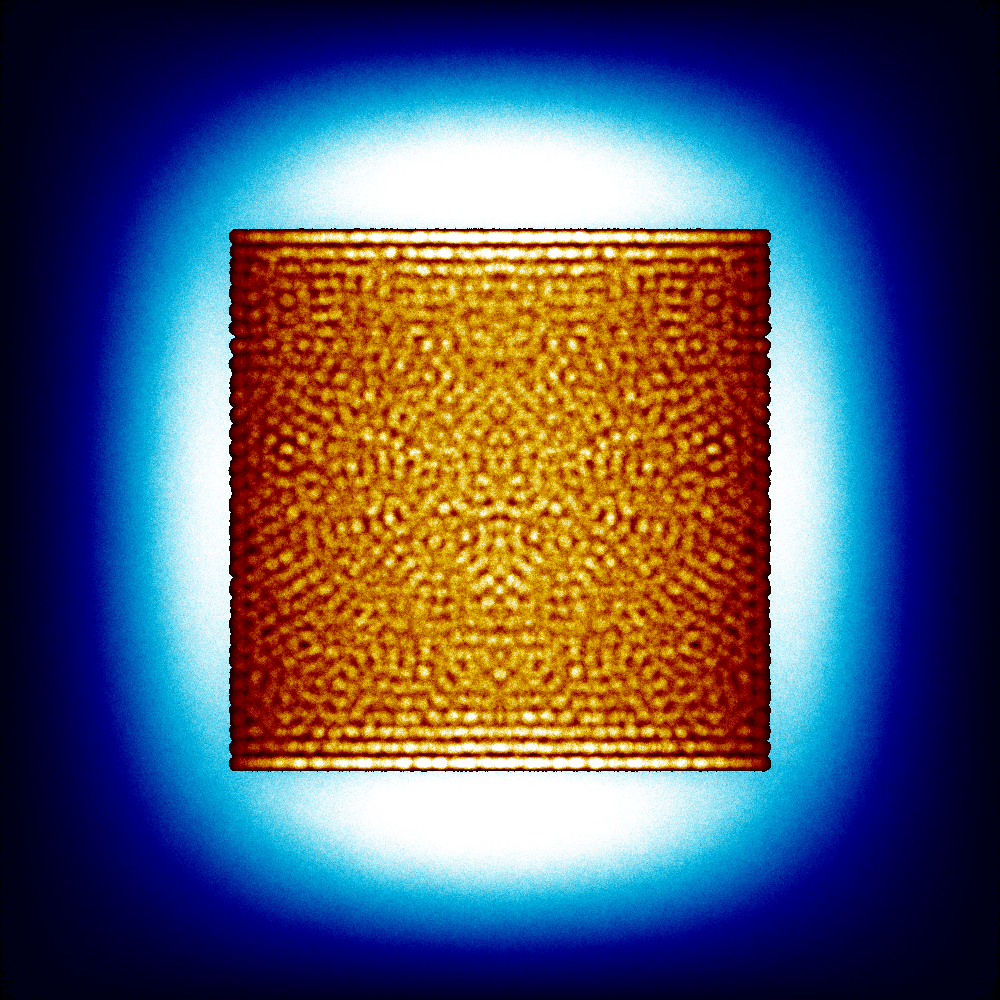
\includegraphics[width=0.95\linewidth]{figures/300-360/300-360-vm}
  \caption{Axial Mesh}
  \label{fig:bstep1}
\end{subfigure}
%
\caption{Sensitivity Analysis: $300^{\circ}$ - $360^{\circ}$}
\label{fig:300-360}
\end{figure}
\begin{figure}[H]
\centering
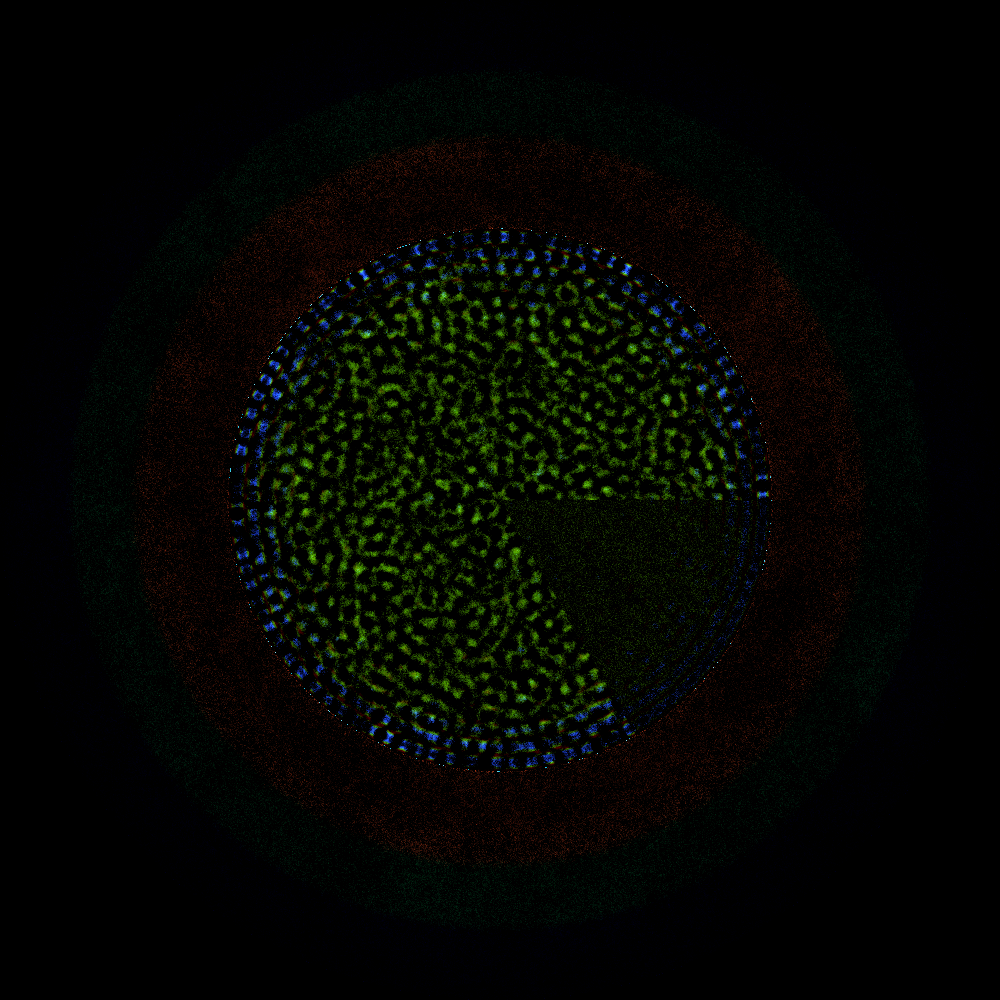
\includegraphics[width=0.6\linewidth]{figures/300-360/diff-300-360}
\caption{An Image Generated by Subtracting \ref{fig:300-360-rm} from \ref{fig:controlb}.}
\label{fig:300-360-diff}
\end{figure}

Figure \ref{fig:300-360} provides fission rate and thermal flux visualization meshes for the symmetry test using the 300 - 360 degree slice.  Figure \ref{fig:300-360-diff} is the result of using image-difference between the control's full-core radial mesh and the symmetry test's mesh.


In each of the image difference results, the section of the core the symmetry assumption  uses --- for example, the portion of Figure \ref{fig:60-120-diff} in the sector from $60^{\circ}$ - $120^{\circ}$ --- is very dark.  This means that this region has very little difference between it and the same sector on the control model result.  The boundaries of these sectors in the image difference are also hard lines, not gradients, which suggests that the neutronics (specifically the fission rate) within and around pebbles closest to the boundary of the sector might not be as significantly impacted by their neighbor pebbles "changing" as expected.  The image difference results also show very little difference in the reflector region, which makes sense, as the reflector is uniform.  However, this does indicate that there wasn't a local peak in thermal flux due to, say, a mass of fresh pebbles in the representative slice.  If there were such a spike, there would likely be repeating regions of brighter "hotspots" in the reflector everywhere \emph{except} the representative sector used in the symmetry assumption.

\section{Appendix B: Shuffle Test}
\label{app-shuf}
Appendix B contains the geometry cross sections, fission rate/thermal flux meshes, and image difference results from the shuffling tests (see \autoref{meth-sens}, Table \ref{table:shuffle})


\begin{figure}[H]
\centering

\begin{subfigure}{0.45\textwidth}
  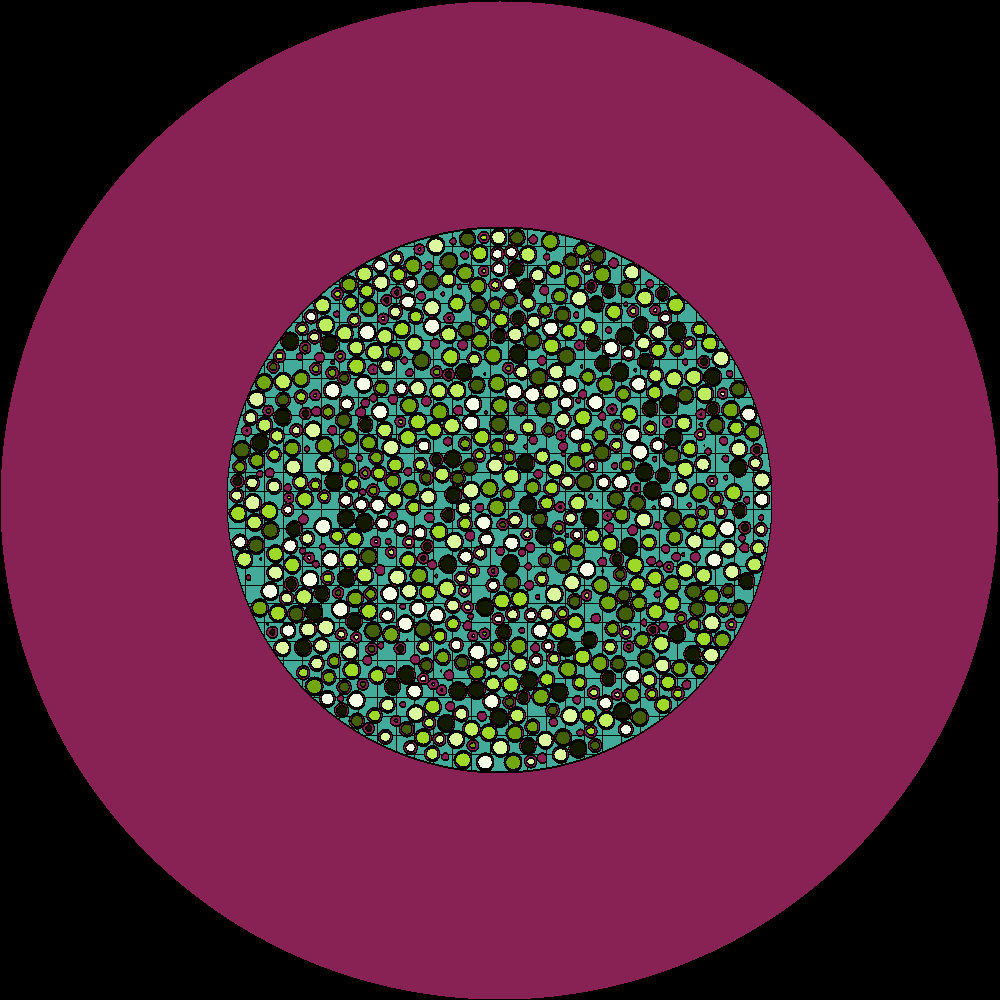
\includegraphics[width=0.95\linewidth]{figures/1234560/1234560-r}
  \caption{Radial Cross Section at y=0}
  \label{fig:1234560-r}
\end{subfigure}%
%
\begin{subfigure}{0.45\textwidth}
  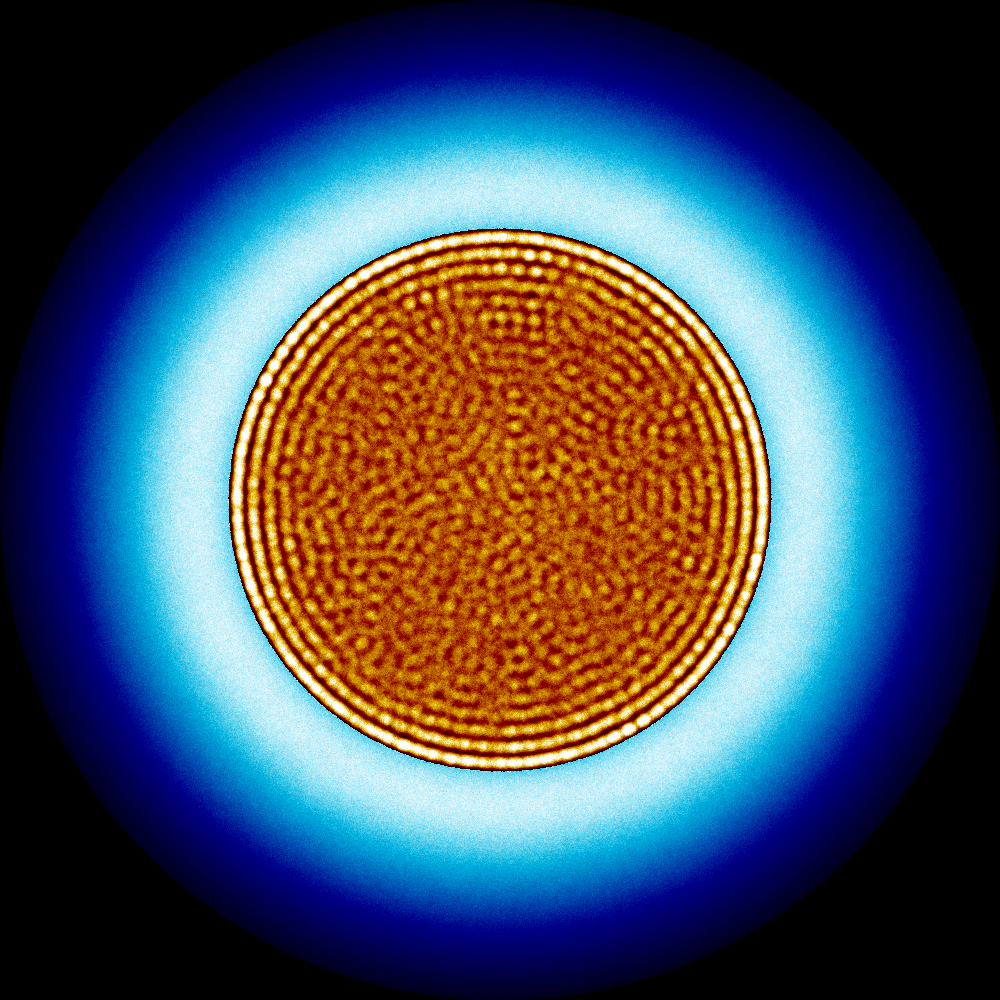
\includegraphics[width=0.95\linewidth]{figures/1234560/1234560-rm}
  \caption{Radial Mesh}
  \label{fig:1234560-rm}
\end{subfigure}

\begin{subfigure}{0.45\textwidth}
  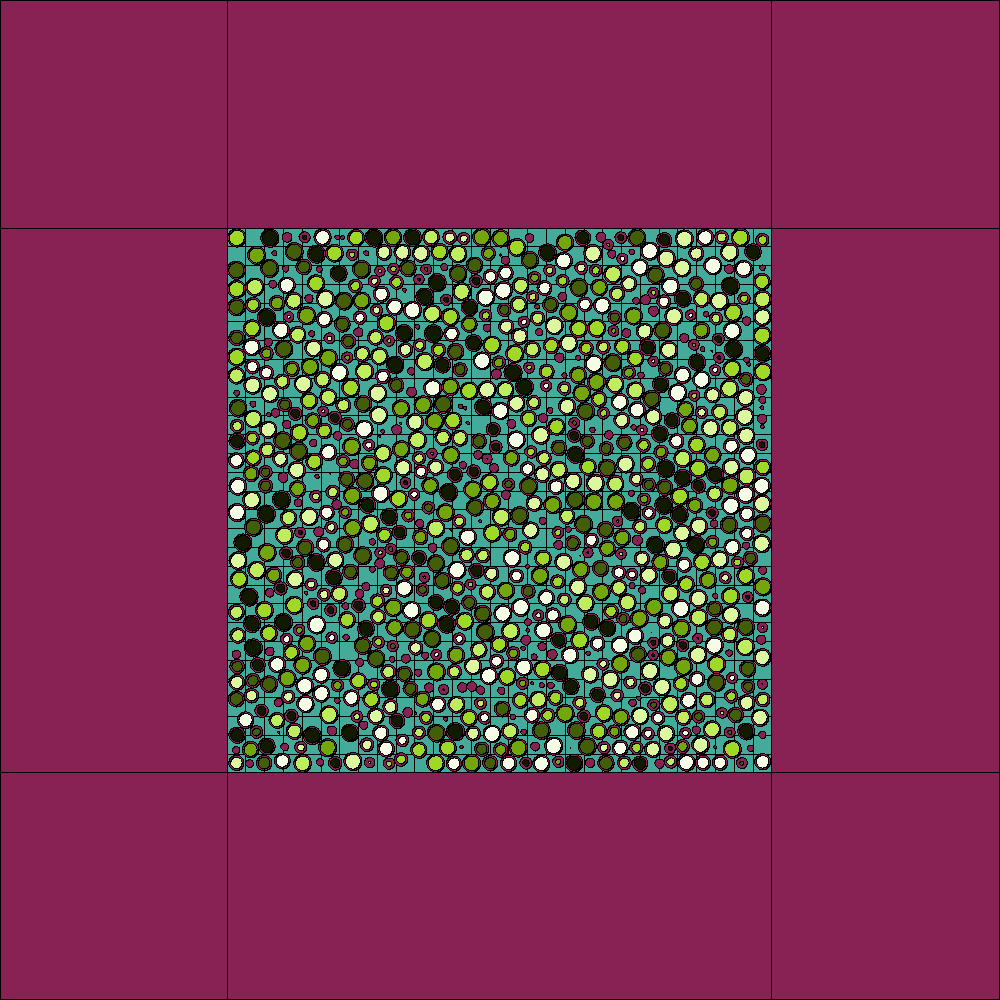
\includegraphics[width=0.95\linewidth]{figures/1234560/1234560-v}
  \caption{Axial Cross Section at z=0 }
  \label{fig:1234560-v}
\end{subfigure}
%
\begin{subfigure}{0.45\textwidth}
  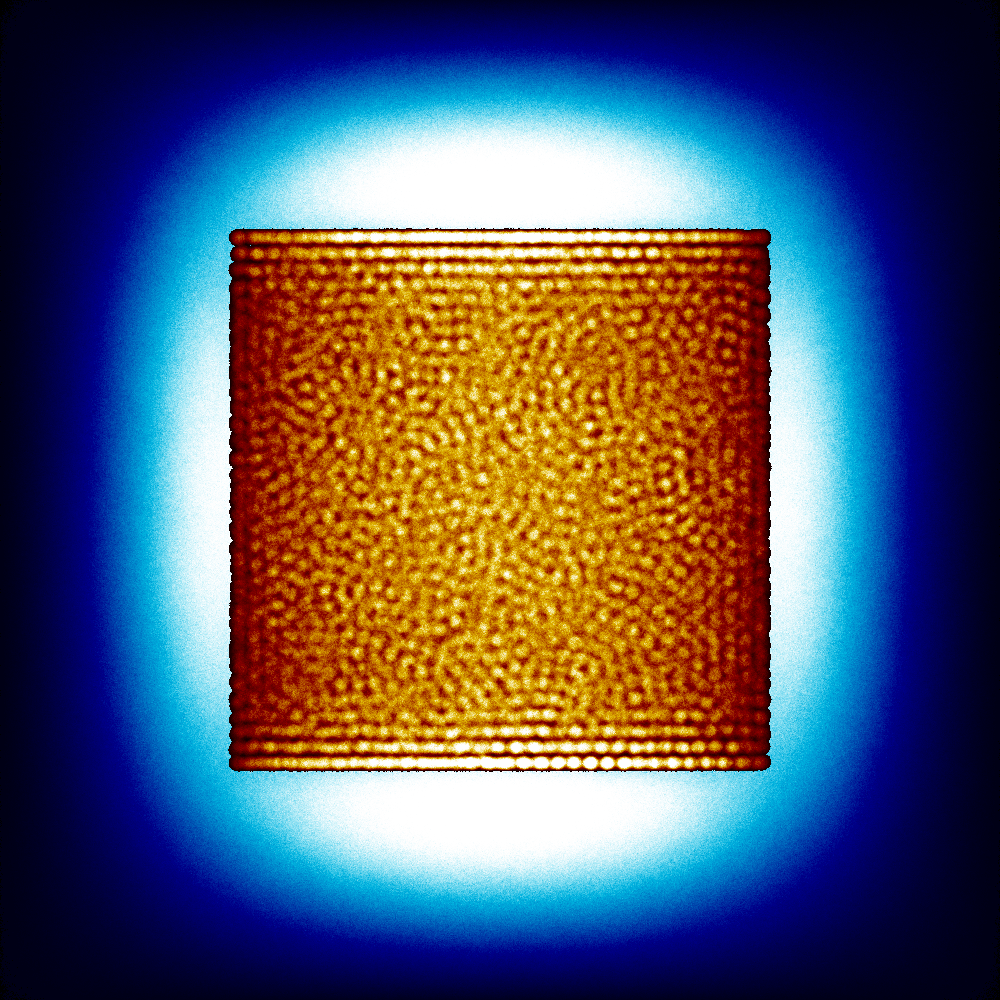
\includegraphics[width=0.95\linewidth]{figures/1234560/1234560-vm}
  \caption{Axial Mesh}
  \label{fig:1234560-vm}
\end{subfigure}
%
\caption{Shuffle Analysis: Run 1}
\label{fig:1234560}
\end{figure}
\begin{figure}[H]
\centering
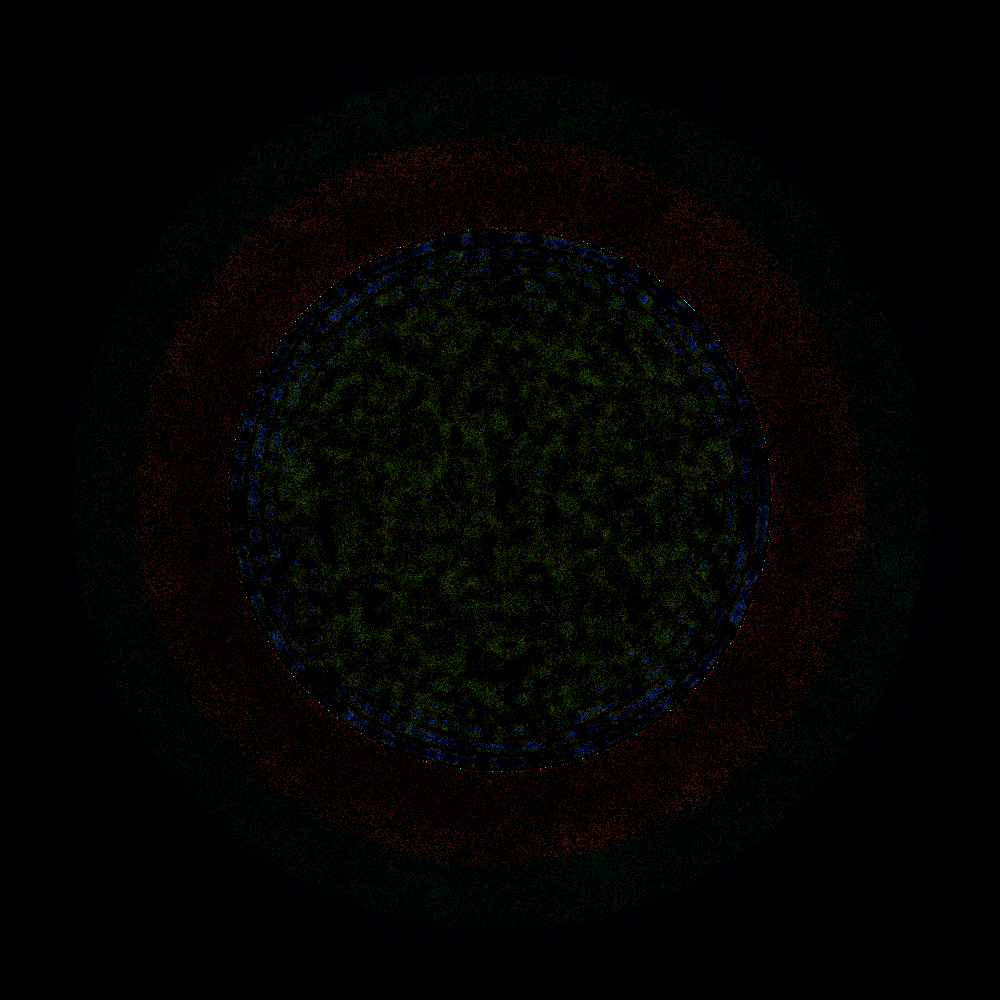
\includegraphics[width=0.6\linewidth]{figures/shuffle/diff-1234560}
\caption{An Image Generated by Subtracting \ref{fig:diff-1234560-rm} from \ref{fig:controlb}.}
\label{fig:diff-1234560}
\end{figure}

Figure \ref{fig:1234560} provides the thermal flux and fission rate meshes and geometric cross sections axially and radially.  Figure \ref{fig:diff-1234560} is the result of the image difference between the full core control mesh and Figure \ref{fig:1234560-rm}.

\begin{figure}[H]
\centering

\begin{subfigure}{0.45\textwidth}
  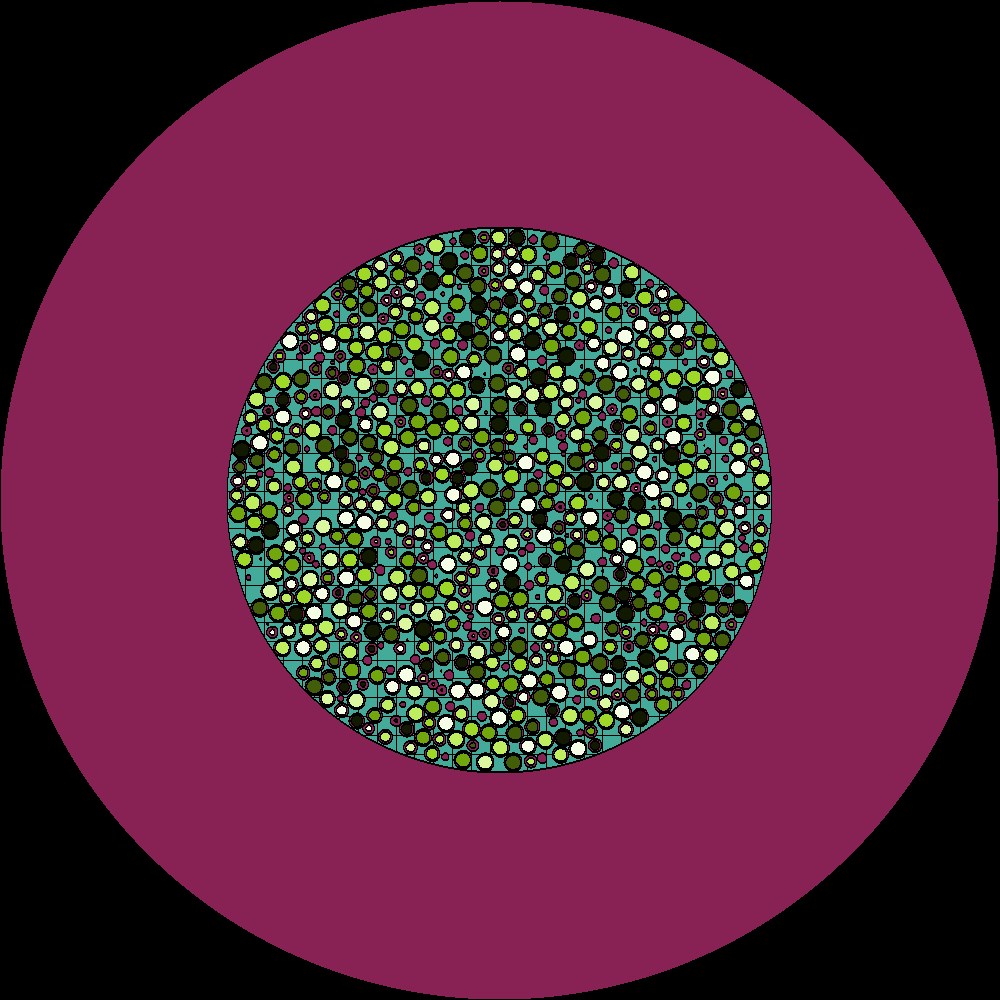
\includegraphics[width=0.95\linewidth]{figures/2345601/2345601-r}
  \caption{Radial Cross Section at y=0}
  \label{fig:2345601-r}
\end{subfigure}%
%
\begin{subfigure}{0.45\textwidth}
  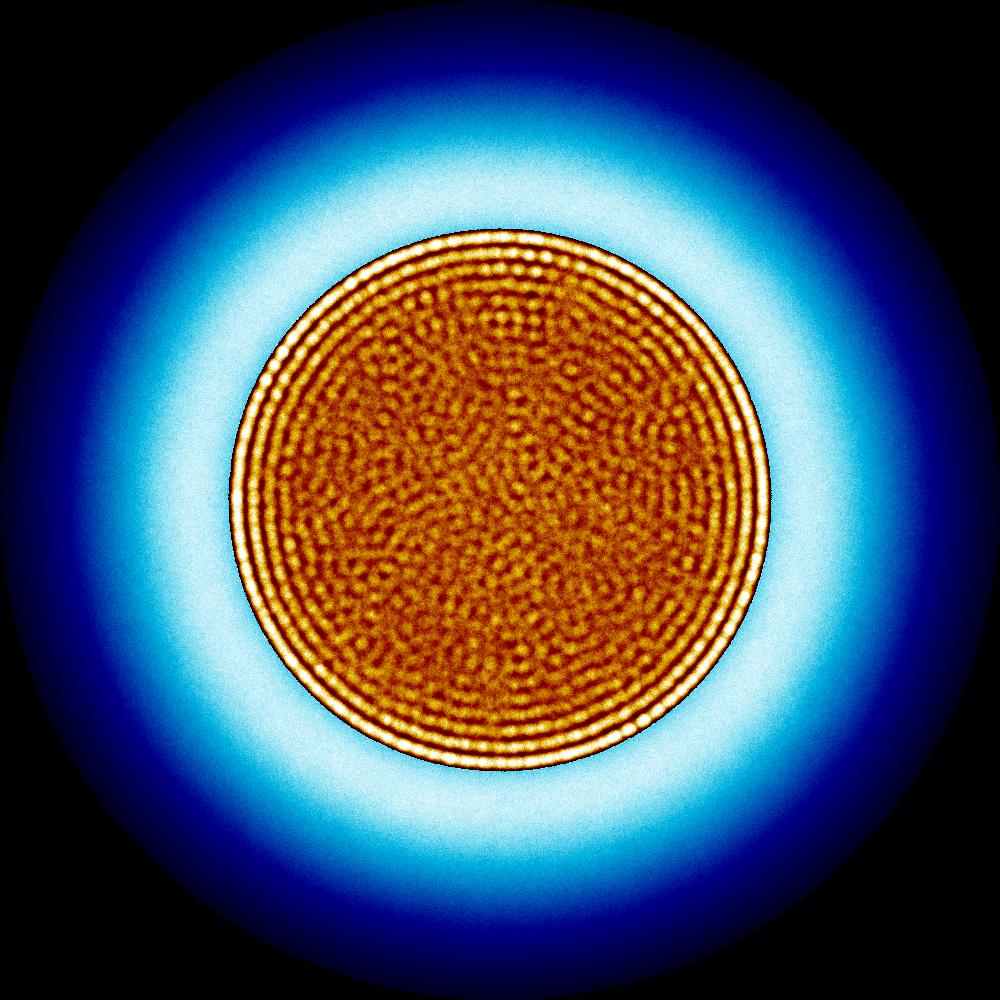
\includegraphics[width=0.95\linewidth]{figures/2345601/2345601-rm}
  \caption{Radial Mesh}
  \label{fig:2345601-rm}
\end{subfigure}

\begin{subfigure}{0.45\textwidth}
  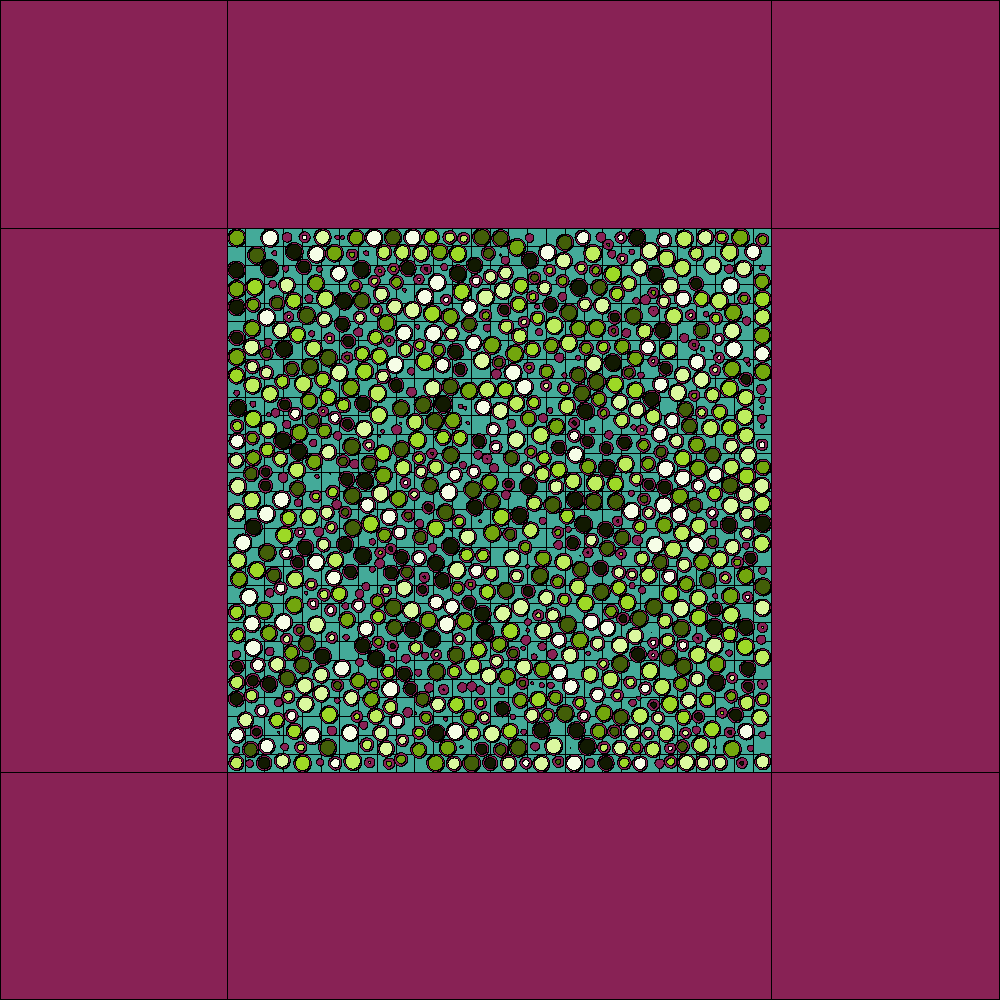
\includegraphics[width=0.95\linewidth]{figures/2345601/2345601-v}
  \caption{Axial Cross Section at z=0 }
  \label{fig:2345601-v}
\end{subfigure}
%
\begin{subfigure}{0.45\textwidth}
  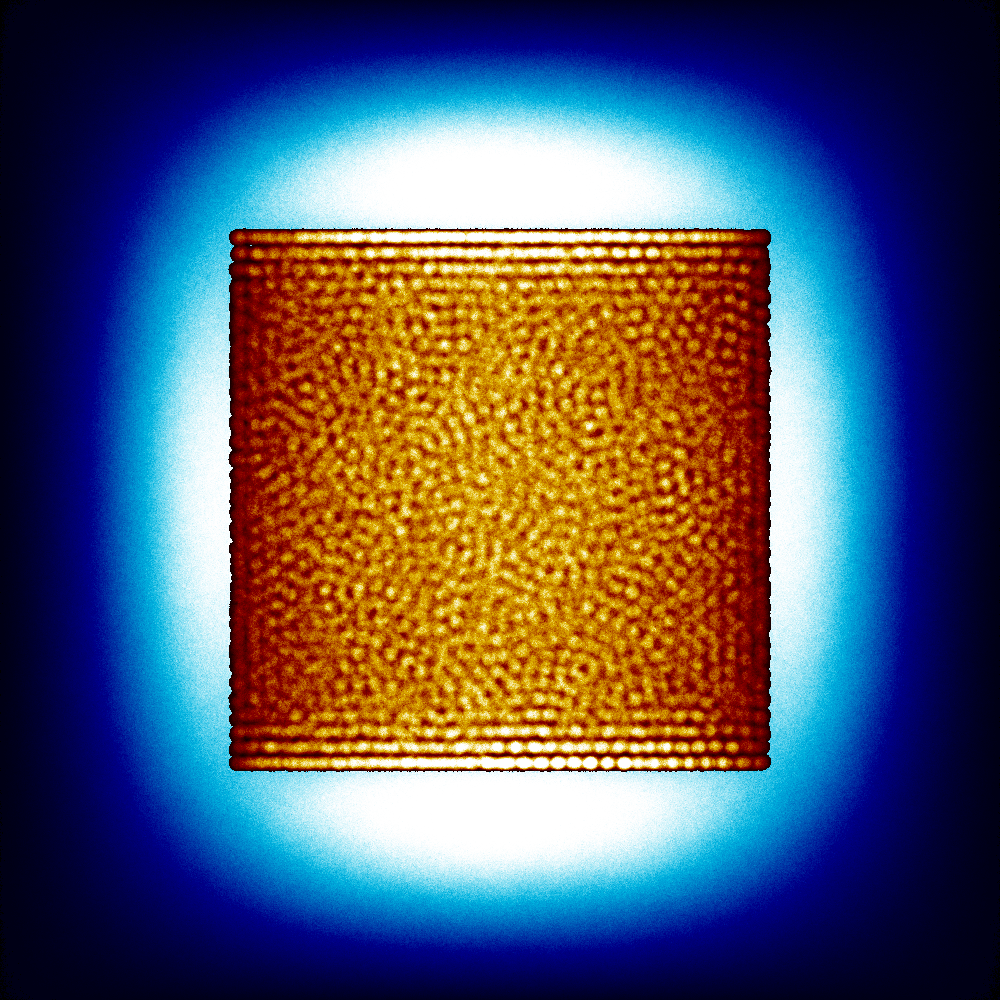
\includegraphics[width=0.95\linewidth]{figures/2345601/2345601-vm}
  \caption{Axial Mesh}
  \label{fig:2345601-vm}
\end{subfigure}
%
\caption{Shuffle Analysis: Run 2}
\label{fig:0-60}
\end{figure}
\begin{figure}[H]
\centering
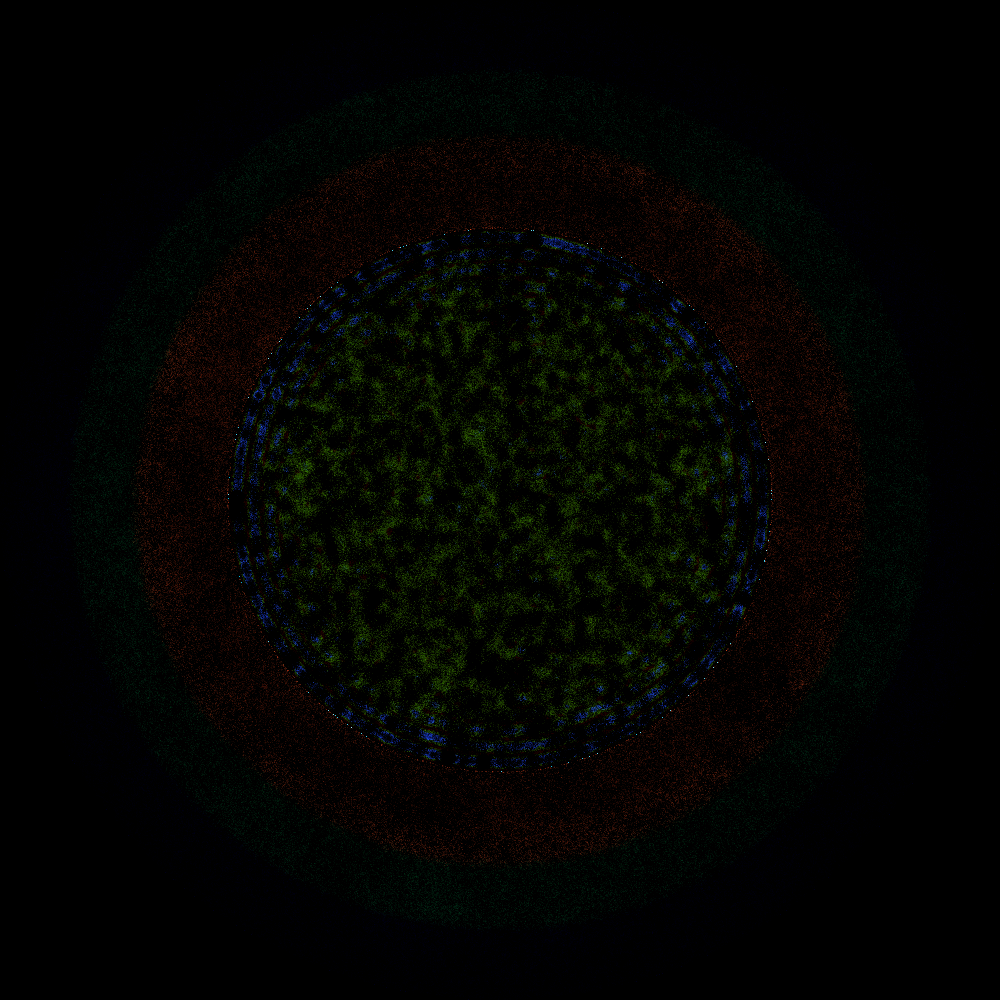
\includegraphics[width=0.6\linewidth]{figures/shuffle/diff-2345601}
\caption{An Image Generated by Subtracting \ref{fig:2345601-rm} from \ref{fig:controlb}.}
\label{fig:diff-2345601}
\end{figure}

Figure \ref{fig:2345601} provides the thermal flux and fission rate meshes and geometric cross sections axially and radially.  Figure \ref{fig:diff-2345601} is the result of the image difference between the full core control mesh and Figure \ref{fig:2345601-rm}.

\begin{figure}[H]
\centering

\begin{subfigure}{0.45\textwidth}
  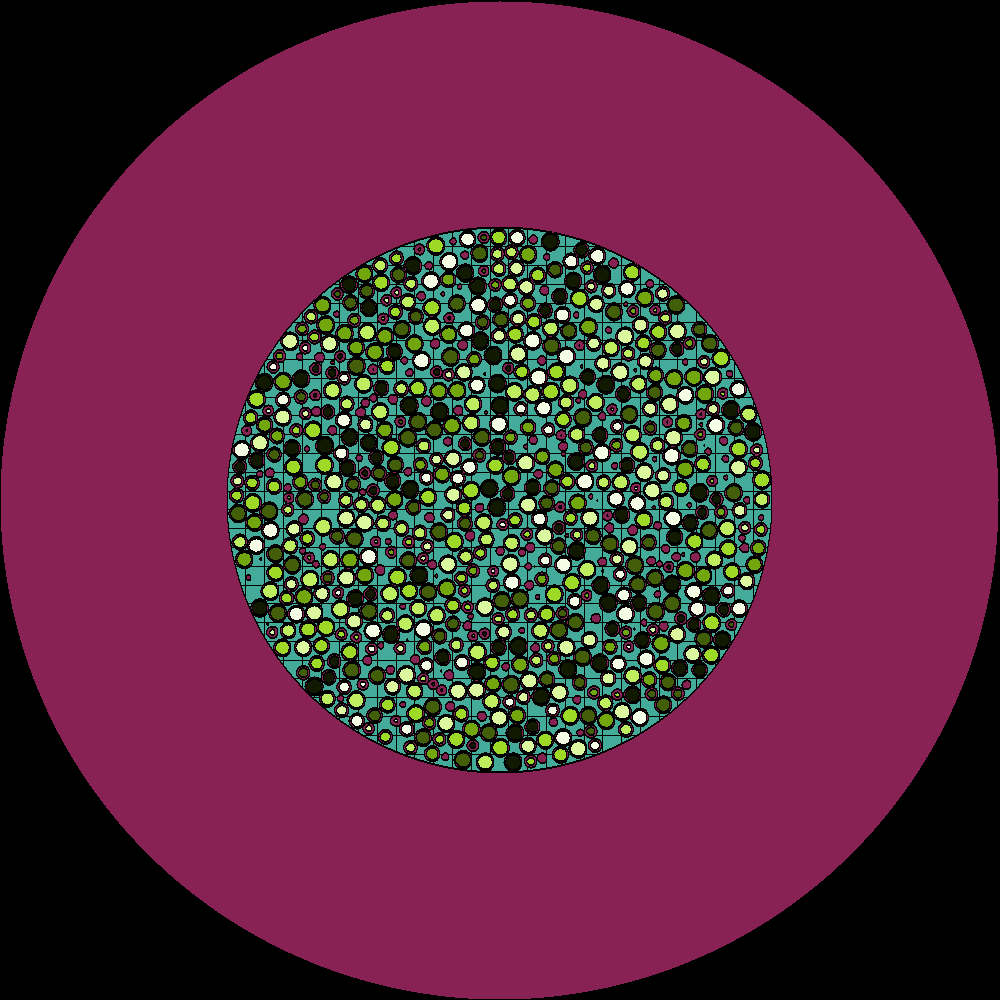
\includegraphics[width=0.95\linewidth]{figures/3456012/3456012-r}
  \caption{Radial Cross Section at y=0}
  \label{fig:3456012-r}
\end{subfigure}%
%
\begin{subfigure}{0.45\textwidth}
  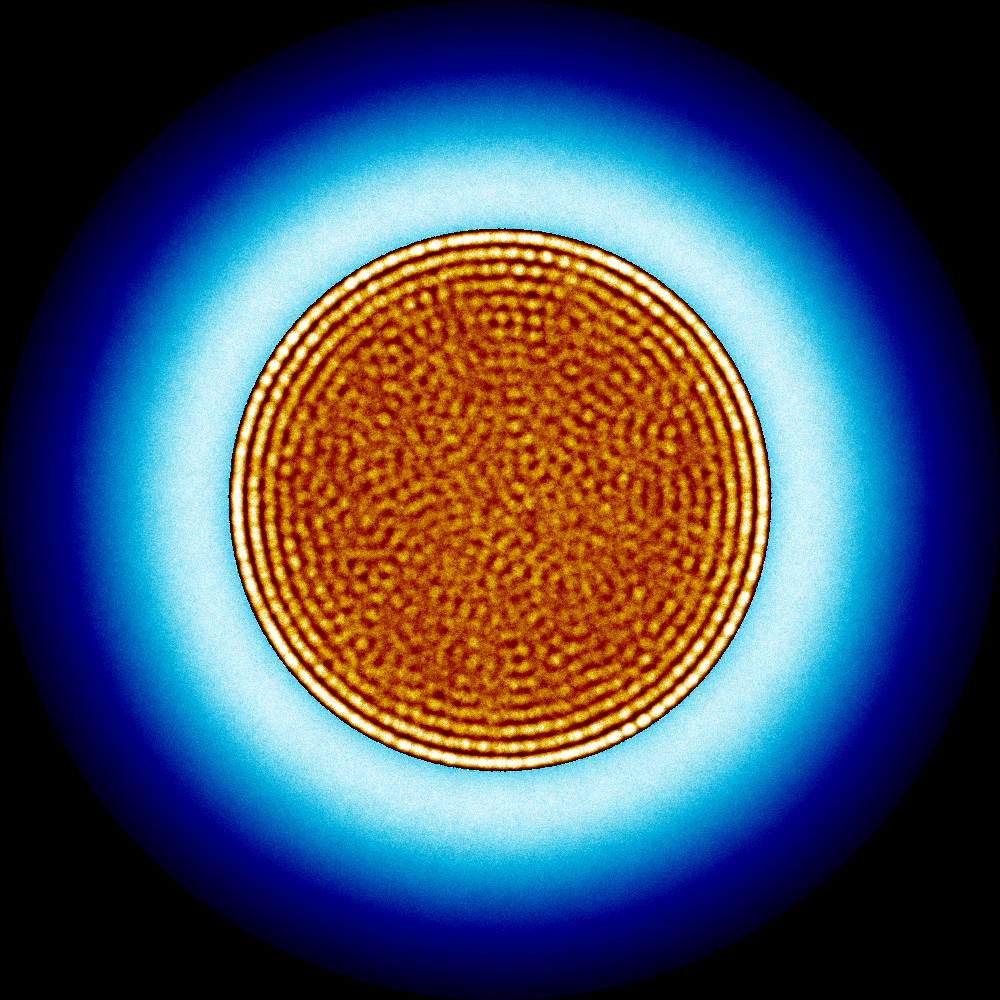
\includegraphics[width=0.95\linewidth]{figures/3456012/3456012-rm}
  \caption{Radial Mesh}
  \label{fig:3456012-rm}
\end{subfigure}

\begin{subfigure}{0.45\textwidth}
  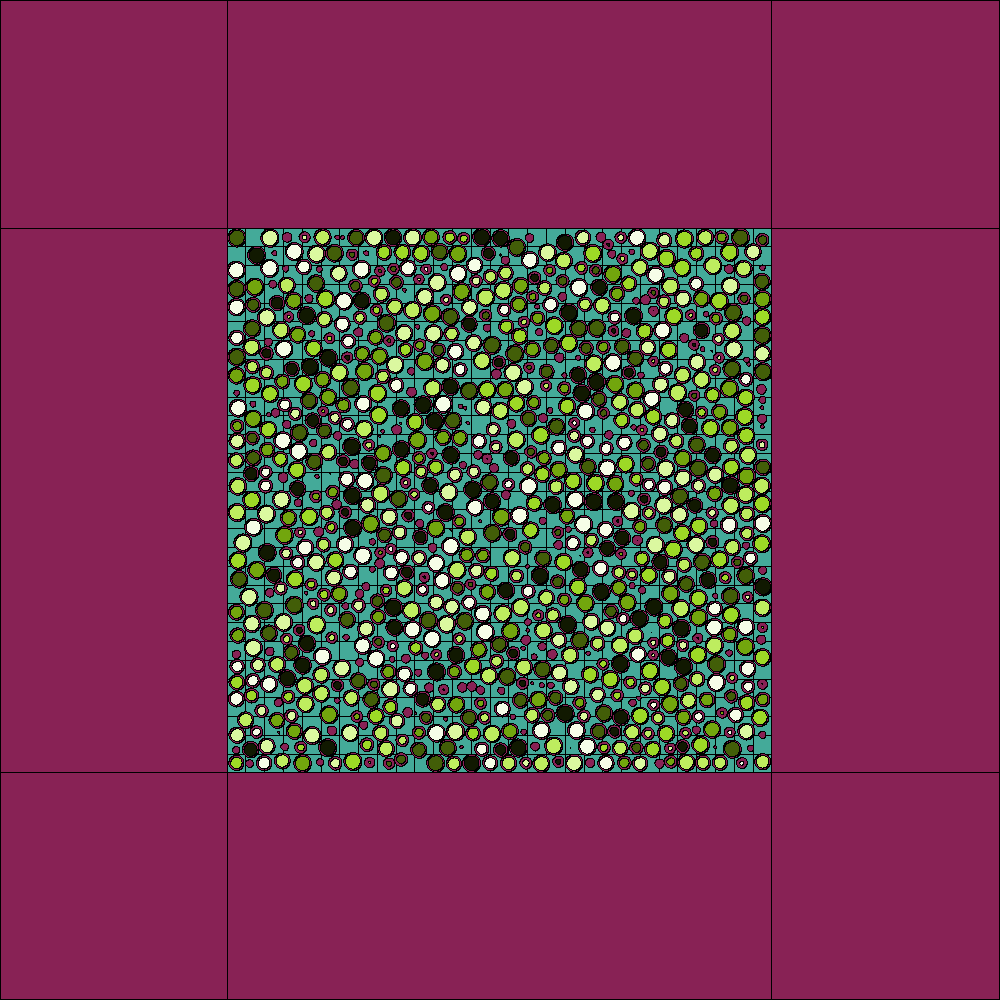
\includegraphics[width=0.95\linewidth]{figures/3456012/3456012-v}
  \caption{Axial Cross Section at z=0 }
  \label{fig:3456012-v}
\end{subfigure}
%
\begin{subfigure}{0.45\textwidth}
  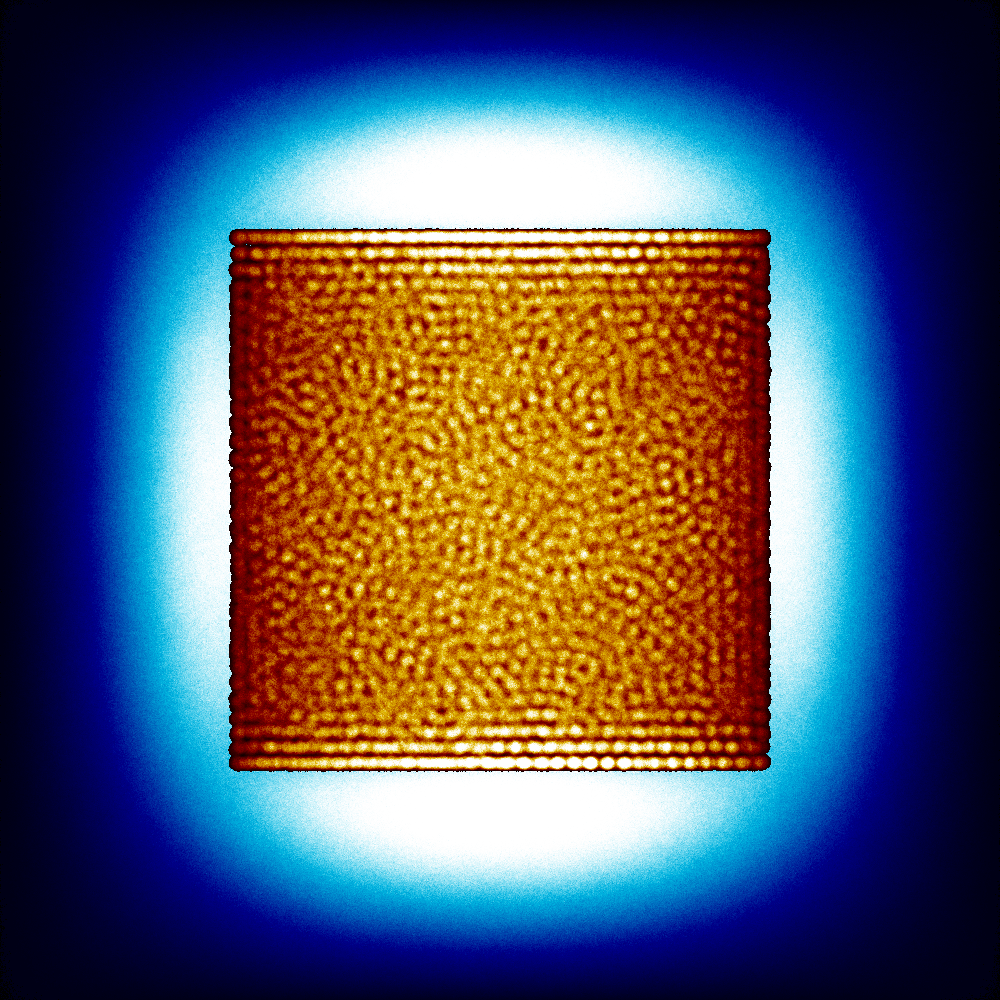
\includegraphics[width=0.95\linewidth]{figures/3456012/3456012-vm}
  \caption{Axial Mesh}
  \label{fig:3456012-vm}
\end{subfigure}
%
\caption{Shuffle Analysis: Run 3}
\label{fig:3456012}
\end{figure}
\begin{figure}[H]
\centering
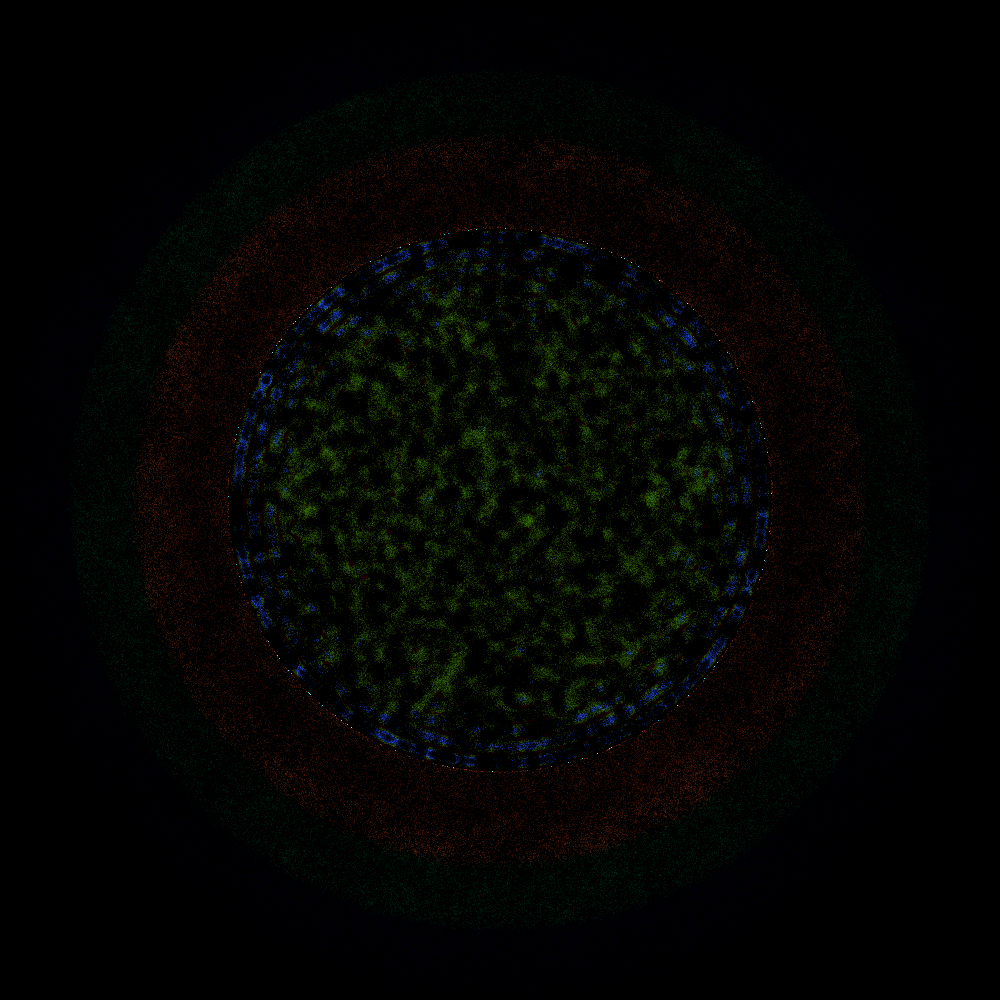
\includegraphics[width=0.6\linewidth]{figures/shuffle/diff-3456012}
\caption{An Image Generated by Subtracting Figure \ref{fig:3456012-rm} from Figure \ref{fig:controlb}.}
\label{fig:diff-3456012}
\end{figure}

Figure \ref{fig:3456012} provides the thermal flux and fission rate meshes and geometric cross sections axially and radially.  Figure \ref{fig:diff-3456012} is the result of the image difference between the full core control mesh and Figure \ref{fig:3456012-rm}.

\begin{figure}[H]
\centering

\begin{subfigure}{0.45\textwidth}
  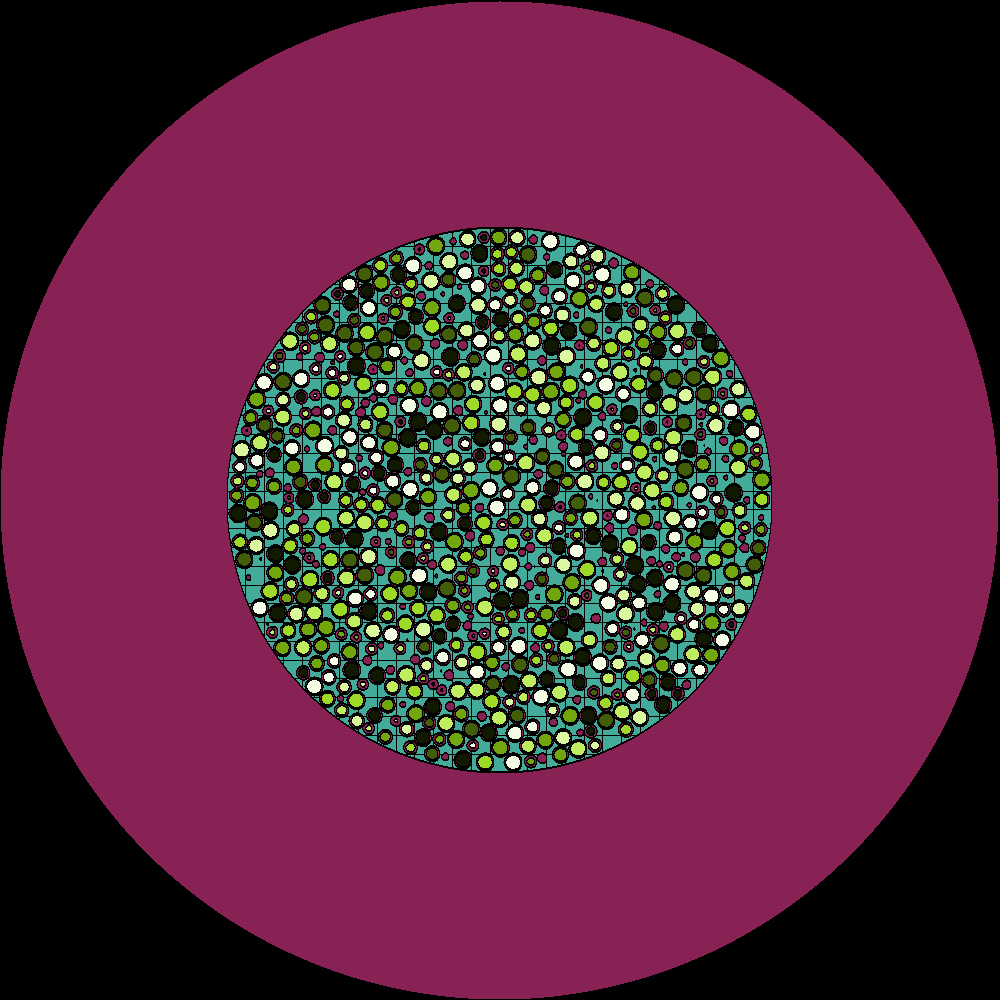
\includegraphics[width=0.95\linewidth]{figures/4560123/4560123-r}
  \caption{Radial Cross Section at y=0}
  \label{fig:4560123-r}
\end{subfigure}%
%
\begin{subfigure}{0.45\textwidth}
  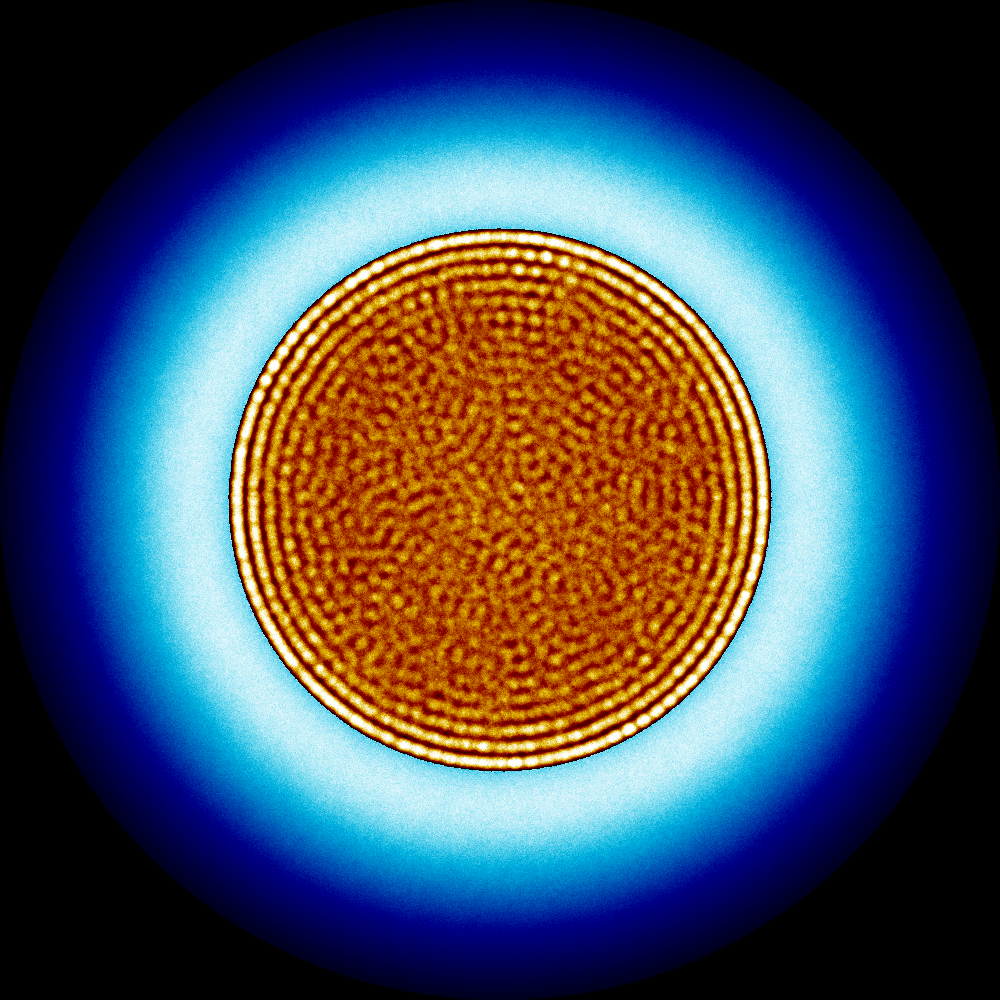
\includegraphics[width=0.95\linewidth]{figures/4560123/4560123-rm}
  \caption{Radial Mesh}
  \label{fig:4560123-rm}
\end{subfigure}

\begin{subfigure}{0.45\textwidth}
  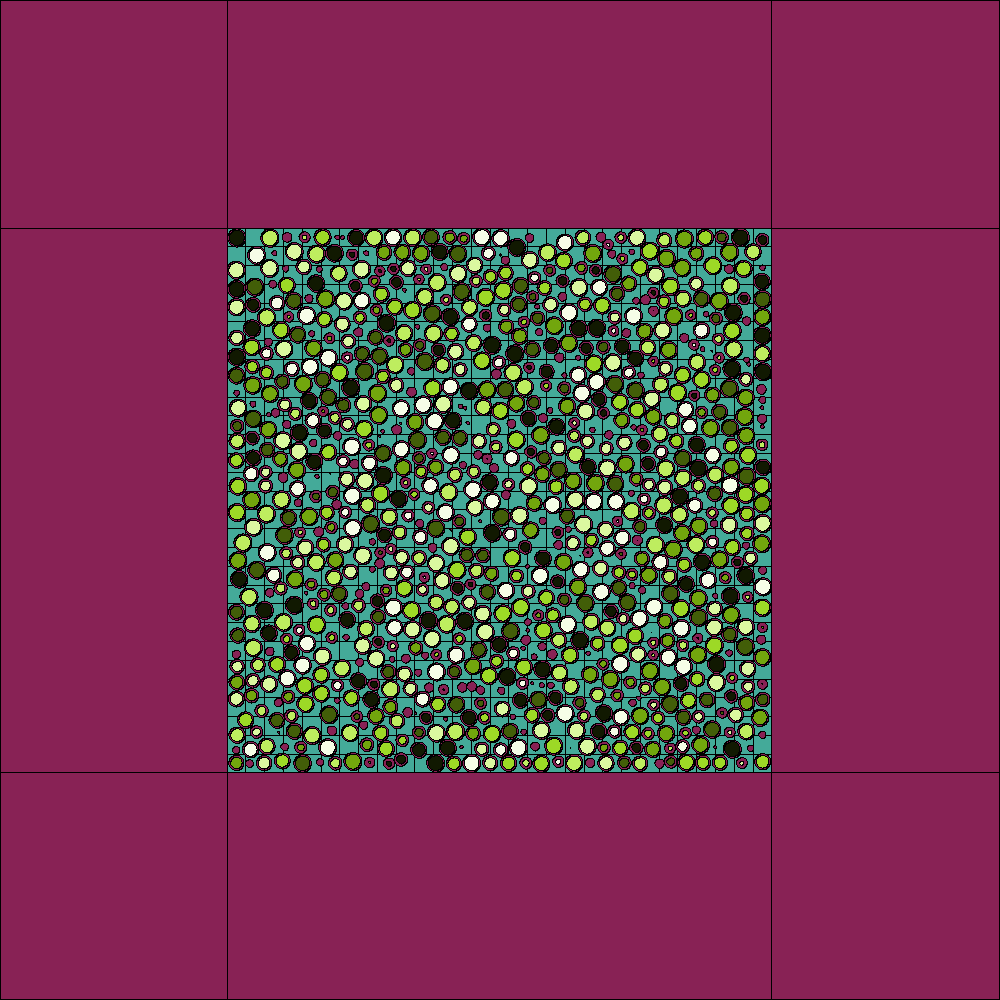
\includegraphics[width=0.95\linewidth]{figures/4560123/4560123-v}
  \caption{Axial Cross Section at z=0 }
  \label{fig:4560123-v}
\end{subfigure}
%
\begin{subfigure}{0.45\textwidth}
  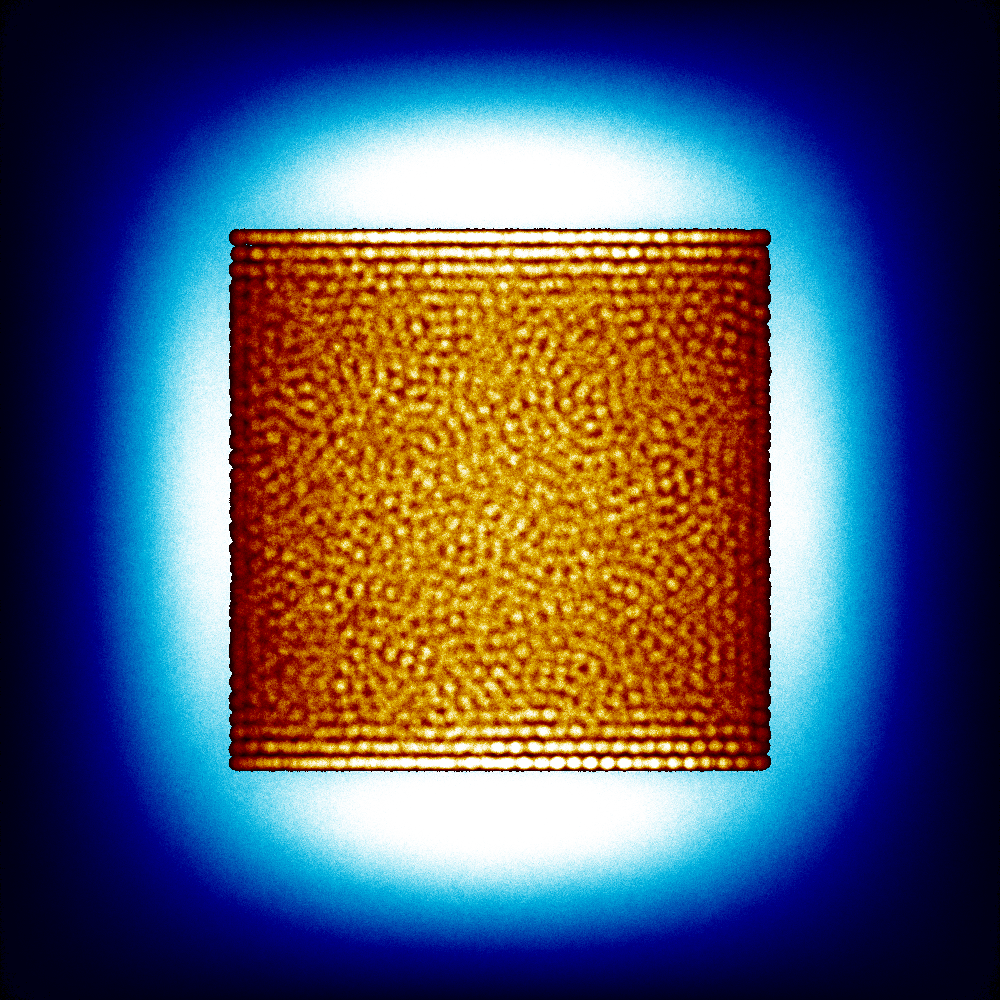
\includegraphics[width=0.95\linewidth]{figures/4560123/4560123-vm}
  \caption{Axial Mesh}
  \label{fig:4560123-vm}
\end{subfigure}
%
\caption{Shuffle Analysis: Run 4}
\label{fig:4560123}
\end{figure}
\begin{figure}[H]
\centering
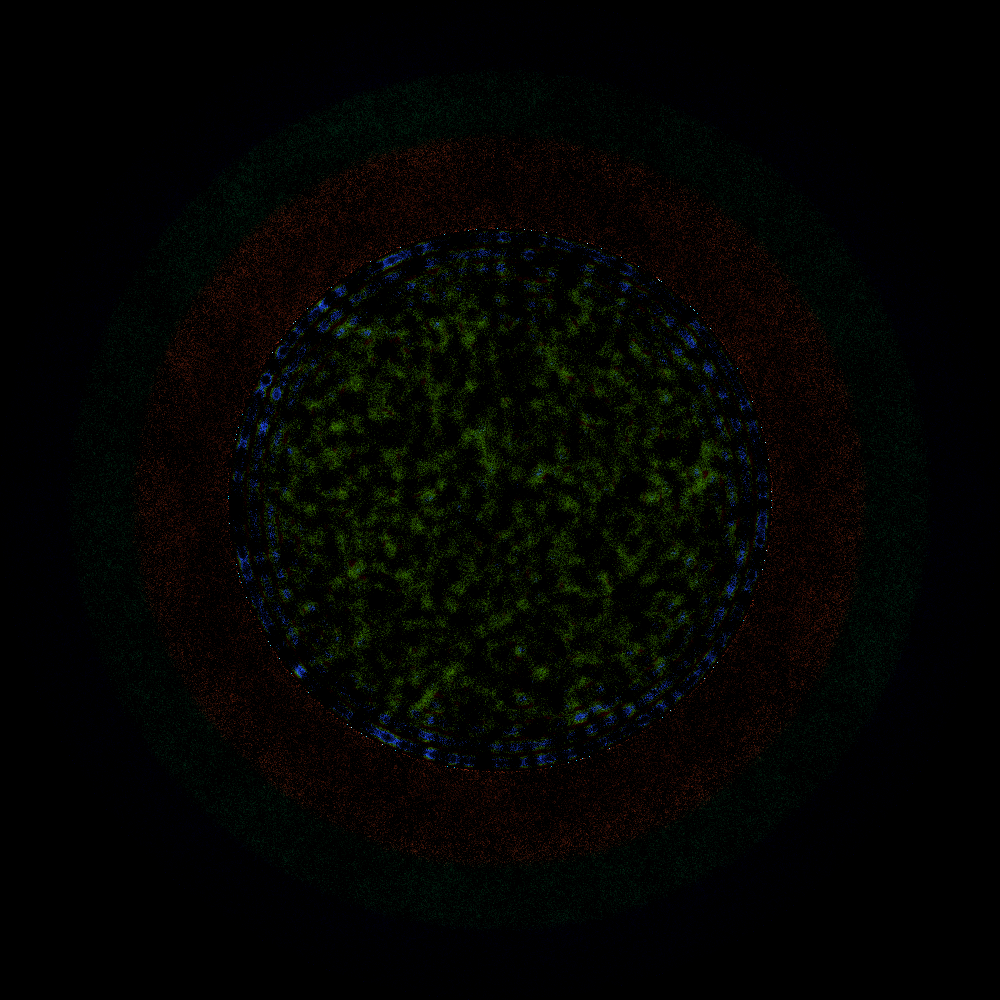
\includegraphics[width=0.6\linewidth]{figures/shuffle/diff-4560123}
\caption{An Image Generated by Subtracting \ref{fig:4560123-rm} from \ref{fig:controlb}.}
\label{fig:diff-4560123}
\end{figure}

Figure \ref{fig:4560123} provides the thermal flux and fission rate meshes and geometric cross sections axially and radially.  Figure \ref{fig:diff-4560123} is the result of the image difference between the full core control mesh and Figure \ref{fig:4560123-rm}.

\begin{figure}[H]
\centering

\begin{subfigure}{0.45\textwidth}
  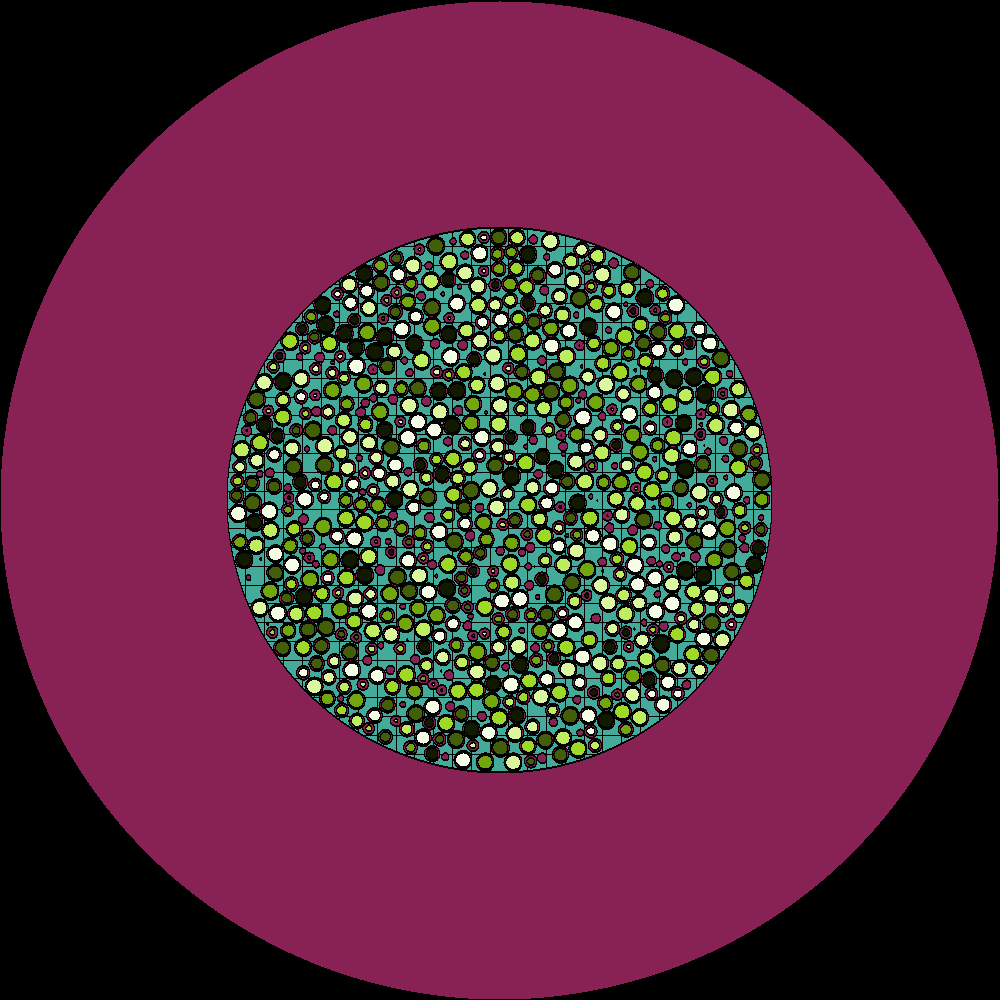
\includegraphics[width=0.95\linewidth]{figures/5601234/5601234-r}
  \caption{Radial Cross Section at y=0}
  \label{fig:5601234-r}
\end{subfigure}%
%
\begin{subfigure}{0.45\textwidth}
  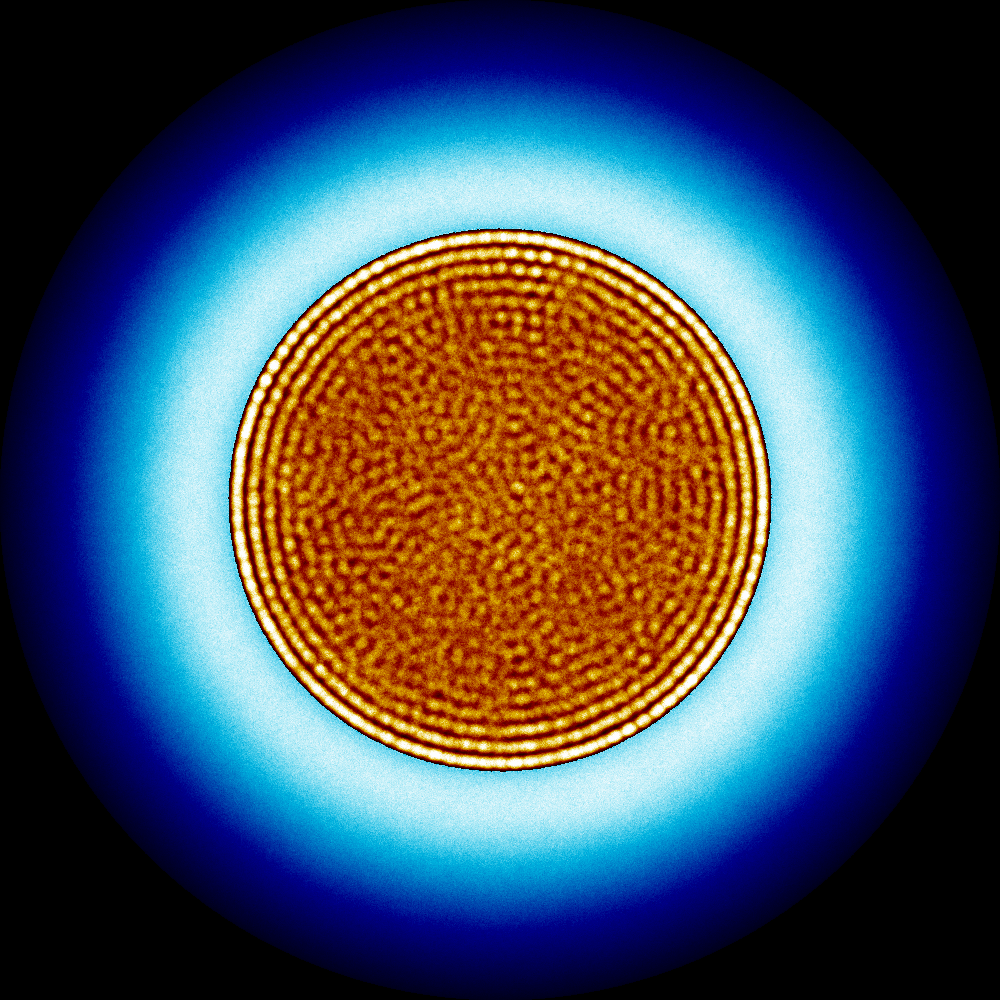
\includegraphics[width=0.95\linewidth]{figures/5601234/5601234-rm}
  \caption{Radial Mesh}
  \label{fig:5601234-rm}
\end{subfigure}

\begin{subfigure}{0.45\textwidth}
  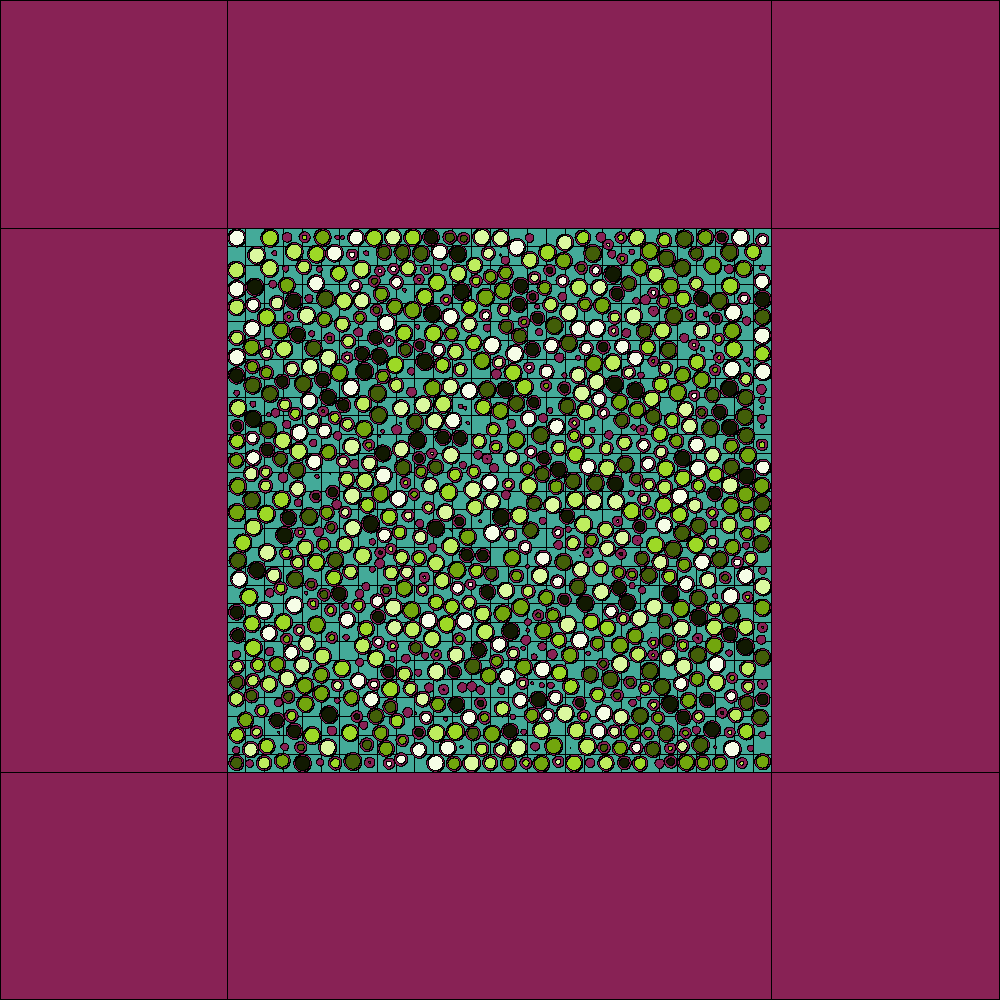
\includegraphics[width=0.95\linewidth]{figures/5601234/5601234-v}
  \caption{Axial Cross Section at z=0 }
  \label{fig:5601234-v}
\end{subfigure}
%
\begin{subfigure}{0.45\textwidth}
  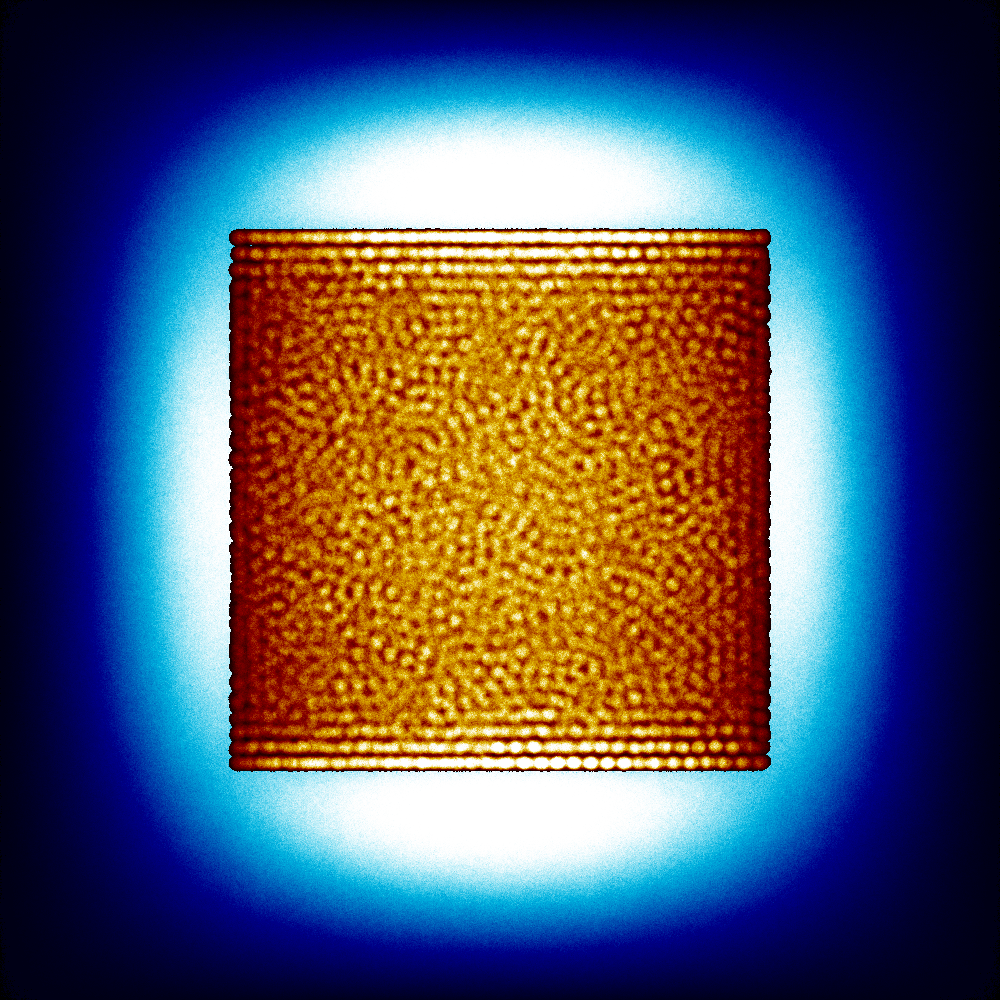
\includegraphics[width=0.95\linewidth]{figures/5601234/5601234-vm}
  \caption{Axial Mesh}
  \label{fig:5601234-vm}
\end{subfigure}
%
\caption{Shuffle Analysis: Run 5}
\label{fig:5601234}
\end{figure}
\begin{figure}[H]
\centering
\includegraphics[width=0.6\linewidth]{figures/shuffle/diff-5601234}
\caption{An Image Generated by Subtracting \ref{fig:diff-5601234-rm} from \ref{fig:controlb}.}
\label{fig:diff-5601234}
\end{figure}

Figure \ref{fig:5601234} provides the thermal flux and fission rate meshes and geometric cross sections axially and radially.  Figure \ref{fig:diff-5601234} is the result of the image difference between the full core control mesh and Figure \ref{fig:5601234-rm}.

\begin{figure}[H]
\centering

\begin{subfigure}{0.45\textwidth}
  \includegraphics[width=0.95\linewidth]{figures/6012345/6012345-r}
  \caption{Radial Cross Section at y=0}
  \label{fig:6012345-r}
\end{subfigure}%
%
\begin{subfigure}{0.45\textwidth}
  \includegraphics[width=0.95\linewidth]{figures/6012345/6012345-rm}
  \caption{Radial Mesh}
  \label{fig:6012345-rm}
\end{subfigure}

\begin{subfigure}{0.45\textwidth}
  \includegraphics[width=0.95\linewidth]{figures/6012345/6012345-v}
  \caption{Axial Cross Section at z=0 }
  \label{fig:6012345-v}
\end{subfigure}
%
\begin{subfigure}{0.45\textwidth}
  \includegraphics[width=0.95\linewidth]{figures/6012345/6012345-vm}
  \caption{Axial Mesh}
  \label{fig:6012345-vm}
\end{subfigure}
%
\caption{Shuffle Analysis: Run 6}
\label{fig:6012345}
\end{figure}
\begin{figure}[H]
\centering
\includegraphics[width=0.6\linewidth]{figures/shuffle/diff-6012345}
\caption{An Image Generated by Subtracting Figure \ref{fig:6012345-rm} from Figure \ref{fig:controlb}.}
\label{fig:diff-6012345}
\end{figure}

Figure \ref{fig:6012345} provides the thermal flux and fission rate meshes and geometric cross sections axially and radially.  Figure \ref{fig:diff-6012345} is the result of the image difference between the full core control mesh and Figure \ref{fig:6012345-rm}.

Comparing the image difference results of Appendix B, the shuffling test, to Appendix A, the symmetry test, shows that the shuffling tests have a weaker effect on the fission rate and thermal flux than the symmetry tests.  The small differences in this particular test would most likely indicate that the core is generally well-mixed, i.e., that each bin in the vertical direction, along the z axis, has each of the 7 fuel compositions represented equally.

There are however, a few hotspots, where small regions show a brighter patch of green.  The best example of this is in the fourth quadrant of Figure \ref{fig:diff-6012345}, near the $270^{\circ}$ line.  Hotspots such as this could be caused by poor mixing, which would make some pebbles occur in higher concentrations (and then cause a larger difference in the shuffle test, when the same region is now dominated by a different burnup) or by the shuffling putting a different pebble burnup in a region of lower or higher flux.  To investigate the source of this, the pebbles in a ~10 cm square column (10 cm in x and y, the height of the reactor in z) around the hotspot were found.  Table \ref{table:10cmpebb} shows the count of each pebble burnup.


\begin{table}[H]
\centering
\caption{Representation of Pebbles by Number of Passes in a 10 cm Square Rectangular Prism Surrounding an Image Difference Hotspot at Approximately x = 11 cm, y = -56 cm}
 \begin{tabularx}{0.35\textwidth}{c  c}
 	\hline
 	Pebble Pass & Number of Pebbles \\
 	\hline
 	Fresh & 20 \\
 	First Pass & 12 \\
 	Second Pass & 13 \\
 	Third Pass & 12 \\
 	Fourth Pass & 10 \\
 	Fifth Pass & 14 \\
 	Sixth Pass & 11 \\
 	\hline
 \end{tabularx}
\label{table:10cmpebb}
\end{table}

When this region was narrowed further, to a ~5 cm region, the poor mixing was more dramatic, as seen in Table \ref{table:5cmpebb}.


\begin{table}[H]
\centering
\caption{Representation of Pebbles by Number of Passes in a 5 cm Square Rectangular Prism Surrounding an Image Difference Hotspot at Approximately x = 11 cm, y = -56 cm}
 \begin{tabularx}{0.35\textwidth}{c  c}
 	\hline
 	Pebble Pass & Number of Pebbles \\
 	\hline
 	Fresh & 10\\
 	First Pass & 3 \\
 	Second Pass & 4 \\
 	Third Pass & 1 \\
 	Fourth Pass & 2 \\
 	Fifth Pass & 2 \\
 	Sixth Pass & 2 \\
 	\hline

 \end{tabularx}
\label{table:5cmpebb}
\end{table}

In the 10 cm square column, fresh pebbles originally make up 21.7\% of all pebbles in the region.  In the 5cm square column that is tighter around the hotspot, fresh pebbles make up 41.7\% of all pebbles.  The hotspot pointed out in Figure \ref{fig:diff-6012345} exists in some degree in Figures \ref{fig:diff-1234560}, \ref{fig:diff-2345601}, \ref{fig:diff-3456012}, \ref{fig:diff-4560123}, and \ref{fig:diff-5601234} --- it is simply brightest in Figure \ref{fig:diff-6012345} because the shuffle scheme corresponding to this Figure \ref{fig:diff-6012345} replaces fresh pebbles with 6-pass pebbles, which have the greatest disparity in burnup.